\documentclass[12pt,dvipdfmx]{beamer}
\usepackage{graphicx}
\DeclareGraphicsExtensions{.pdf}
\DeclareGraphicsExtensions{.eps}
\graphicspath{{out/tex/svg/}}
\usepackage{listings}
\usepackage{fancybox}
\usepackage{hyperref}
\usepackage{color}

\newcommand{\plusequal}{\mbox{\tt\ += }}
\newcommand{\minusequal}{\mbox{\tt\ -= }}
\newcommand{\divequal}{\mbox{\tt\ /= }}
\newcommand{\plusplus}{\mbox{\tt\ ++ }}

%\usepackage{transparent}
\newcommand\transparent[1]{}

%%%%%%%%%%%%%%%%%%%%%%%%%%%
%%% themes
%%%%%%%%%%%%%%%%%%%%%%%%%%%
%\usetheme{Szeged} 
\usetheme{Madrid}

%% no navigation bar
% default boxes Bergen Boadilla Madrid Pittsburgh Rochester
%% tree-like navigation bar
% Antibes JuanLesPins Montpellier
%% toc sidebar
% Berkeley PaloAlto Goettingen Marburg Hannover Berlin Ilmenau Dresden Darmstadt Frankfurt Singapore Szeged
%% Section and Subsection Tables
% Copenhagen Luebeck Malmoe Warsaw

%%%%%%%%%%%%%%%%%%%%%%%%%%%
%%% innerthemes
%%%%%%%%%%%%%%%%%%%%%%%%%%%
% \useinnertheme{circles}	% default circles rectangles rounded inmargin

%%%%%%%%%%%%%%%%%%%%%%%%%%%
%%% outerthemes
%%%%%%%%%%%%%%%%%%%%%%%%%%%
% outertheme
% \useoutertheme{default}	% default infolines miniframes smoothbars sidebar sprit shadow tree smoothtree


%%%%%%%%%%%%%%%%%%%%%%%%%%%
%%% colorthemes
%%%%%%%%%%%%%%%%%%%%%%%%%%%
\usecolortheme{seahorse}
%% special purpose
% default structure sidebartab 
%% complete 
% albatross beetle crane dove fly seagull 
%% inner
% lily orchid rose
%% outer
% whale seahorse dolphin

%%%%%%%%%%%%%%%%%%%%%%%%%%%
%%% fontthemes
%%%%%%%%%%%%%%%%%%%%%%%%%%%
\usefonttheme{serif}  
% default professionalfonts serif structurebold structureitalicserif structuresmallcapsserif

%%%%%%%%%%%%%%%%%%%%%%%%%%%
%%% generally useful beamer settings
%%%%%%%%%%%%%%%%%%%%%%%%%%%
% 
\AtBeginDvi{\special{pdf:tounicode EUC-UCS2}}
% do not show navigation
\setbeamertemplate{navigation symbols}{}
% show page numbers
\setbeamertemplate{footline}[frame number]


%%%%%%%%%%%%%%%%%%%%%%%%%%%
%%% define some colors for convenience
%%%%%%%%%%%%%%%%%%%%%%%%%%%

\newcommand{\mido}[1]{{\color{green}#1}}
\newcommand{\mura}[1]{{\color{purple}#1}}
\newcommand{\ore}[1]{{\color{orange}#1}}
\newcommand{\ao}[1]{{\color{blue}#1}}
\newcommand{\aka}[1]{{\color{red}#1}}

\setbeamercolor{ex}{bg=cyan!20!white}

%%%%%%%%%%%%%%%%%%%%%%%%%%%
%%% how to typset code
%%%%%%%%%%%%%%%%%%%%%%%%%%%

\lstset{language = C,
numbers = left,
numberstyle = {\tiny \emph},
numbersep = 10pt,
breaklines = true,
breakindent = 40pt,
frame = tlRB,
frameround = ffft,
framesep = 3pt,
rulesep = 1pt,
rulecolor = {\color{blue}},
rulesepcolor = {\color{blue}},
flexiblecolumns = true,
keepspaces = true,
basicstyle = \ttfamily\scriptsize,
identifierstyle = ,
commentstyle = \it\scriptsize,
stringstyle = ,
showstringspaces = false,
tabsize = 4,
escapechar=\@,
}

\title{How to Solve Complex Problems in Parallel \\
(Divide and Conquer \\ {\em and\/} Task Parallelism)}
\institute{}
\author{Kenjiro Taura}
\date{}

\AtBeginSection[] % Do nothing for \section*
{
\begin{frame}
\frametitle{Contents}
\tableofcontents[currentsection,currentsubsection]
\end{frame}
}

\AtBeginSubsection[] % Do nothing for \section*
{
\begin{frame}
\frametitle{Contents}
\tableofcontents[currentsection,currentsubsection]
\end{frame}
}

\begin{document}
\maketitle

%%%%%%%%%%%%%%%%%%%%%%%%%%%%%%%%%% 
\begin{frame}
\frametitle{Contents}
\tableofcontents
\end{frame}

\section{Introduction}
%%%%%%%%%%%%%%%%% 
\begin{frame}
\frametitle{Goals}
learn:
\begin{itemize}
\item the power of divide and conquer paradigm

\item how to write and parallelize
  divide and conquer algorithms with task parallelism

\item and how to reason about the speedup
  of task parallel programs
  \begin{itemize}
  \item work
  \item critical path length
  \item Greedy Scheduler theorem
  \end{itemize}
\end{itemize}
\end{frame}

%%%%%%%%%%%%%%%%%
\iffalse
\begin{frame}
\frametitle{Hands-on exercise next week}

\begin{itemize}
\item please bring your laptop with SSH
\item details on the necessary 
  preparation are (hopefully) on the home page
  until the weekend
\end{itemize}

\begin{center}

\includegraphics[width=0.3\textwidth]{out/pdf/svg/nicubunu_Comic_characters_Operator.pdf}  
\end{center}
\end{frame}
\fi

%%%%%%%%%%%%%%%%% 
\begin{frame}[fragile]
\frametitle{Divide and conquer algorithms}
\begin{itemize}
\item ``Divide and conquer'' is the single
  most important design paradigm of algorithms
\item []
\begin{lstlisting}[basicstyle=\scriptsize]
answer solve(@$D$@) {
  if (trivial(@$D$@)) {
    return trivially_solve(@$D$@);
  } else {
    @$D_1, \ldots , D_k$@ = @\ao{divide}@(@$D$@); // divide the problem into sub problems
    @$a_1$@ = solve(@$D_1$@); @$\ldots$@; @$a_k$@ = solve(@$D_k$@); // solve them
    return @\ao{combine}@(@$a_1$@, ..., @$a_k$@); // combine sub answers
  }
}
\end{lstlisting}
\end{itemize}

\def\svgwidth{\textwidth}
{\tiny\input{out/tex/svg/dc.pdf_tex}}

\end{frame}

%%%%%%%%%%%%%%%%% 
\begin{frame}
\frametitle{Benefits of ``divide and conquer'' thinking}
Divide and conquer \ldots
\begin{itemize}
\item often helps you \ao{\em come up with} an algorithm

\item is easy to program, with \ao{\em recursions}

\item is often easy to \ao{\em parallelize}, once
  you have a recursive formulation
  and a parallel programming language that
  supports it (\ao{\em task parallelism})

\item often has a good \ao{\em locality} of
  reference, both in serial and parallel execution
\end{itemize}
\end{frame}


%%%%%%%%%%%%%%%%% 
\begin{frame}
\frametitle{Some examples}
\begin{itemize}
\item quick sort, merge sort
\item matrix multiply, LU factorization, eigenvalue
\item FFT, polynomial multiply, big int multiply
\item maximum segment sum, find median 
\item $k$-d tree
\item \ldots
\end{itemize}
\end{frame}


%%%%%%%%%%%%%%%%%%%%%%%%%%%%%%%%%% 
\section{An example :  $k$-d tree construction}
%%%%%%%%%%%%%%%%%%%%%%%%%%%%%%%%%% 

%%%%%%%%%%%%%%%%% 
\subsection{$k$-d tree}
%%%%%%%%%%%%%%%%% 

%%%%%%%%%%%%%%%%% 
\begin{frame}
\frametitle{$k$-d tree}
\begin{itemize}
\item A data structure to hierarchically organize
  points to facilitate ``nearest neighbor'' or ``proxymity'' searches,
  usually in 2D or 3D space
\item Each node represents a rectangular region
\end{itemize}

\begin{center}
\def\svgwidth{0.5\textwidth}
\input{out/tex/svg/tree300.pdf_tex}  
\end{center}
\end{frame}


%%%%%%%%%%%%%%%%% 
\begin{frame}
\frametitle{$k$-d tree construction}
\begin{columns}
\begin{column}{0.65\textwidth}
\begin{itemize}
\item Input: 
  \begin{itemize}
  \item \ao{$P$}: an array of points (no particular order)
  \item \ao{$R$}: a bounding box of $P$
  \end{itemize}
\item Output:
  \begin{itemize}
  \item \ao{$t$}: a $k$-d tree for $P$
  \end{itemize}
\item Properties $t$ must satisfy
  \begin{enumerate}
  \item<2-> each leaf has $\leq c$ points
  \item<3-> each internal node has one point of its own plus one or two children
  \item<3-> each internal node is split into two subspaces by a line passing through its point
  \item<4-> axis to split a node perpendicular to is chosen alternately
    (first the $x$-axis, then the $y$-axis, and so on)
  \end{enumerate}
\end{itemize}
\end{column}

\begin{column}{0.35\textwidth}
\def\svgwidth{0.6\textwidth}
\only<1>{\input{out/tex/svg/kdtree_leaf0.pdf_tex}}%
\only<2->{Leaf: 

\input{out/tex/svg/kdtree_leaf.pdf_tex}}

\only<1-2>{\input{out/tex/svg/kdtree_internal0.pdf_tex}}%
\only<3->{Internal: \input{out/tex/svg/kdtree_internal.pdf_tex}}

\only<1-3>{\input{out/tex/svg/kdtree_split0.pdf_tex}}%
\only<4>{\input{out/tex/svg/kdtree_split1.pdf_tex}}%
\only<5>{\input{out/tex/svg/kdtree_split2.pdf_tex}}%
\only<6>{\input{out/tex/svg/kdtree_split3.pdf_tex}}%
\only<7->{\input{out/tex/svg/kdtree_split4.pdf_tex}}
\end{column}
\end{columns}
\end{frame}

%%%%%%%%%%%%%%%%% 
\begin{frame}
\frametitle{How to build a $k$-d tree}
Possible strategies:

\begin{itemize}
\item<1->an insertion-based method
  \begin{itemize}
  \item define a method to add a single point into a tree
  \item start from an empty tree and add all points into it
  \end{itemize}

\item<2->\ao{a divide and conquer method}
\end{itemize}
\end{frame}

\iffalse
%%%%%%%%%%%%%%%%% 
\begin{frame}[fragile]
\frametitle{Insertion-based method}

\begin{lstlisting}
/* insert point p into node n */
insert(n, p) {
  if (|n->P| + 1 <= threshold) {
    /* add p to this node and we are done */
    add(n->P, p);
  } else if (|n->P| + 1 == threshold) {
    /* n was leaf and now borns children */
    s = @\mura{\tt find\_pivot}@(n->P, n->depth % D);
    R0,R1 = @\mura{\tt split\_rect}@(n->R, n->depth % D, s.pos[n->depth % D]);
    P0,P1 = @\mura{\tt partition}@(n->P, n->depth % D, s.pos[n->depth % D]);
    /* n becomes an internal node */
    s->P = { s };
    s->c[0] = make_leaf(P0, R0, n->depth + 1);
    s->c[1] = make_leaf(P1, R0, n->depth + 1);
  } else {
    c = find the child that covers p's position;
    insert(c, p);
  }
}  
\end{lstlisting}

\begin{lstlisting}
/* build a tree for points P in region R */
build(P, R) {
  n = make_leaf({}, R, 0);
  for p in P {
    insert(n, p);
  }
  return n;
}
\end{lstlisting}
\end{frame}
\fi

%%%%%%%%%%%%%%%%% 
\begin{frame}
\frametitle{divide and conquer method}
\begin{columns}
\begin{column}{0.55\textwidth}
\begin{itemize}
\item<1-> to build a tree for a rectangle $R$ and points $P$ in $R$,
\item<2-> choose a ``pivot'' $p \in P$ through which to split $R$, and
\item<3-> partition $P$ into $P_0 + \{ p \} + P_1$ where,
  \begin{itemize}
  \item if we split perpendicular to the $x$-axis,
  \item $P_0$ : points whose $x$ coodinate $<$ $p$'s
  \item $P_1$ : points whose $x$ coodinate $\geq$ $p$'s (except $p$)
  \end{itemize}
\end{itemize}
\end{column}
  
\begin{column}{0.45\textwidth}
\begin{center}
\def\svgwidth{\columnwidth}
\only<1>{\input{out/tex/svg/kdtree_at_work_0.pdf_tex}}%
\only<2>{\input{out/tex/svg/kdtree_at_work_1.pdf_tex}}%
\only<3>{\input{out/tex/svg/kdtree_at_work_2.pdf_tex}}%
\only<4>{\input{out/tex/svg/kdtree_at_work_3.pdf_tex}}
\end{center}
\end{column}
\end{columns}
\end{frame}

%%%%%%%%%%%%%%%%% 
\begin{frame}[fragile]
\frametitle{divide and conquer method}
\begin{itemize}
\item []
\begin{lstlisting}
/* build a k-d tree for a set of points P in a rectangular region R and return 
   the root of the tree. the node is at depth, so it should split along 
   (depth % D)th axis */
@\ao{\tt build}@(P, R, depth) {
  if (|P| == 0) {
    return 0; /* empty */
  } else if (|P| <= threshold) {
    /* small enough; leaf */
    return make_leaf(P, R, depth);
  } else {
    /* find a point whose coordinate to split is near the median */
    p = @\mura{\tt find\_pivot}@(P, depth % D);
    /* split R into two sub-rectangles */
    R0,R1 = @\mura{\tt split\_rect}@(R, depth % D, p.pos[depth % D]);
    /* partition P by their coodinate lower/higher than p's coordinate */
    P0,P1 = @\mura{\tt partition}@(P - { p }, depth % D, p.pos[depth % D]);
    /* build a tree for each rectangle */
    n0 = @\ao{\tt build}@(P0, R0, depth + 1);
    n1 = @\ao{\tt build}@(P1, R1, depth + 1);
    /* return a node having n0 and n1 as its children */
    return make_node(p, n0, n1, depth);
  }
}
\end{lstlisting}
\end{itemize}
\end{frame}


%%%%%%%%%%%%%%%%% 
\begin{frame}[fragile]
\frametitle{Notes on subprocedures}

\begin{itemize}
\item $p = $ \mura{\tt find\_pivot}($P$, $d$)
  \begin{itemize}
  \item find a point $\in P$ whose $d$th coordinate
    is (close to) the median value among all points in $P$
  \item sample a few points and choose the median 
    \ao{$\Rightarrow O(1)$}
  \end{itemize}

\item $R_0,R_1 = $ \mura{\tt split\_rect}($R$, $d$, $c$)
  \begin{itemize}
  \item split a rectangular region $R$ by a (hyper-)plane
    ``$d$th coordinate $= c$''
  \item just make two rectangular regions 
    \ao{$\Rightarrow O(1)$}
  \end{itemize}

\item $P_0,P_1 = $ \mura{\tt partition}($P$, $d$, $c$)
  \begin{itemize}
  \item partition a set of points $P$ into two subsets $P_0$
    ($d$th coordinate $< c$) and $P_1$ ($d$th coordinate $\geq c$)
  \item \ao{$\Rightarrow O(|P|)$}
  \end{itemize}
\end{itemize}
\end{frame}


%%%%%%%%%%%%%%%%%%%%%%%%%%%%%%%%%% 
\section{Parallelizing divide and conquer algorithms}
%%%%%%%%%%%%%%%%%%%%%%%%%%%%%%%%%% 

%%%%%%%%%%%%%%%%%%%%%%%%%%%%%%%%%% 
%\subsection{Basics}
%%%%%%%%%%%%%%%%% 
\begin{frame}
\frametitle{Parallelizing divide and conquer}
\begin{itemize}
\item Divide and conquer algorithms are easy to
  parallelize if the programming language/library
  supports asynchronous recursive calls 
  (\aka{\em task parallel\/} systems)
  \begin{itemize}
  \item OpenMP task constructs ({\tt \#pragma omp parallel, master, task, taskwait})
  \item Intel Threading Building Block (TBB)
  \item Cilk, CilkPlus
  \end{itemize}

%\item we use TBB in the following because of its 
%  performance portability
\end{itemize}

\begin{center}
%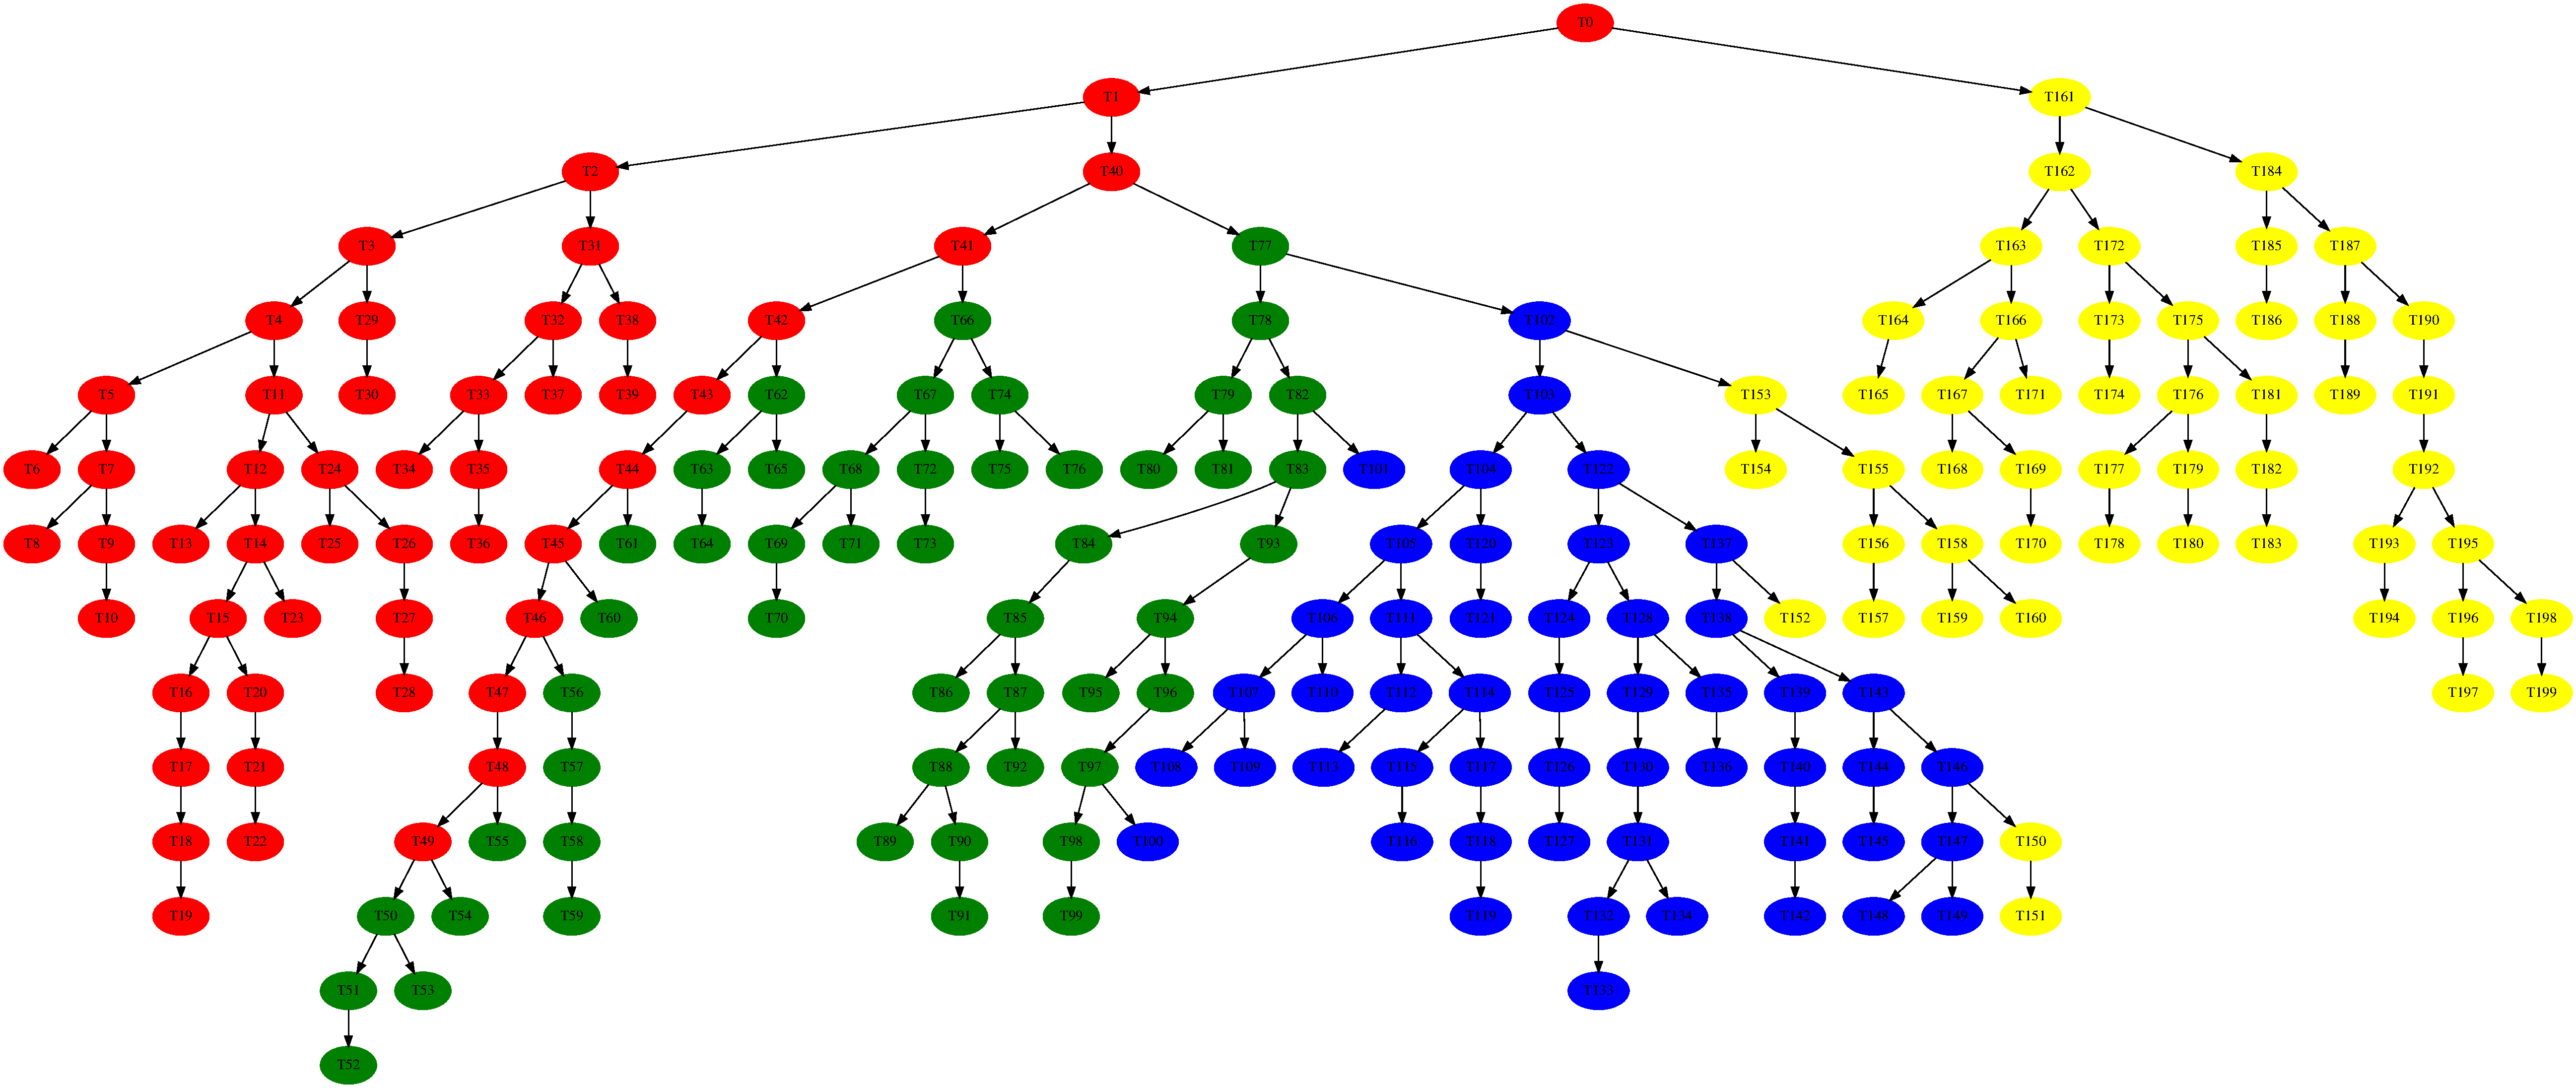
\includegraphics[width=0.8\textwidth]{out/pdf/svg/randtree.pdf}
\end{center}
\end{frame}

%%%%%%%%%%%%%%%%% 
\begin{frame}[fragile]
\frametitle{Parallelizing $k$-d tree construction with tasks}
\begin{itemize}
\item it's as simple as doing two recursions in parallel!
\item e.g., with OpenMP tasks
\item []
\begin{lstlisting}
build(P, R, depth) {
  if (|P| == 0) {
    return 0; /* empty */
  } else if (|P| <= threshold) {
    return make_leaf(P, R, depth);
  } else {
    p = find_pivot(P, depth % D);
    R0,R1 = split_rect(R, depth % D, p.pos[depth % D]);
    P0,P1 = partition(P - { p }, depth % D, p.pos[depth % D]);
@\ao{\texttt{\#pragma omp task shared(n0)}}@
    n0 = build(P0, R0, depth + 1);
@\ao{\texttt{\#pragma omp task shared(n1)}}@
    n1 = build(P1, R1, depth + 1);
@\ao{\texttt{\#pragma omp taskwait}}@
    return make_node(p, n0, n1, depth);
  }
}
\end{lstlisting}
\item cumbersome to parallelize with only parallel loops
\end{itemize}
\end{frame}


%%%%%%%%%%%%%%%%% 
\begin{frame}
\frametitle{Note: tasks and GPU}
\begin{itemize}
\item task parallelism (e.g., OpenMP {\tt \#pragma omp task}) is a great tool to implement divide-and-conquer, \ao{on CPUs}
\item \aka{on GPUs}, the implementation status is unclear and far from done
  \begin{itemize}
  \item NVIDIA HPC SDK (nvc/nvc++) : not supported at all (writing {\tt task} pragmas within {\tt target} region results in compile-time error
  \item LLVM (clang/clang++) : compilation succeeds (at least for simple programs), but how tasks are distributed across CUDA-threads or SMs is uncertain
  \end{itemize}
\item there are inherent challenges around mapping dynamically created tasks onto the SIMT execution model of GPUs
\item never expect it ``just works'' (more bruntly, avoid it altogether, at least for now)
\end{itemize}
\end{frame}


\iffalse
%%%%%%%%%%%%%%%%%%%%%%%%%%%%%%%%%% 
\subsection{Intel TBB}
%%%%%%%%%%%%%%%%% 
\begin{frame}[fragile]
\frametitle{Task parallelism in Intel TBB}
\begin{itemize}
\item we use Intel TBB as a specific example of task parallel
  systems, primarily because of its compiler-independence
\item consider executing the following two calls in parallel
\begin{lstlisting}
    n0 = build(P0, R0, depth + 1);
    n1 = build(P1, R1, depth + 1);
\end{lstlisting}
%    @$\mbox{\ao{gemm}}(A_1, B, C_1);$@
%    @$\mbox{\ao{gemm}}(A_2, B, C_2);$@
\item in TBB, this can be expressed by:
\begin{lstlisting}
    @\ao{\texttt{tbb::task\_group tg}}@;
    @\ao{\texttt{tg.run([\&] \{}}@ n0 = build(P0, R0, depth + 1); @\ao{\texttt \})}@;
    n1 = build(P1, R1, depth + 1);
    @\ao{\texttt{tg.wait()}}@;
\end{lstlisting}
%    // execute @$\mbox{gemm}(A_1, B, C_1)$@ with tasks
%    tg.run([&] { @$\mbox{\ao{gemm}}(A_1, B, C_1);$@ }); // create a task
%    @$\mbox{\ao{gemm}}(A_2, B, C_2);$@

\item note: you can, but do not have to, create a task for the second recursion
\end{itemize}
\end{frame}


%%%%%%%%%%%%%%%%% 
\begin{frame}[fragile]
\frametitle{Parallelizing $k$-d tree construction with TBB}
\begin{itemize}
\item []
\begin{lstlisting}
build(P, R, depth) {
  if (|P| == 0) {
    return 0; /* empty */
  } else if (|P| <= threshold) {
    return make_leaf(P, R, depth);
  } else {
    p = find_pivot(P, depth % D);
    R0,R1 = split_rect(R, depth % D, p.pos[depth % D]);
    P0,P1 = partition(P - { p }, depth % D, p.pos[depth % D]);
    @\ao{\texttt{tbb::task\_group tg}}@;
    @\ao{\texttt{tg.run([\&] \{}}@ n0 = build(P0, R0, depth + 1); @\ao{\texttt \})}@;
    n1 = build(P1, R1, depth + 1);
    @\ao{\texttt{tg.wait()}}@;
    return make_node(p, n0, n1, depth);
  }
}
\end{lstlisting}
\end{itemize}
\end{frame}


%%%%%%%%%%%%%%%%% 
\begin{frame}[fragile]
\frametitle{A summary of \texttt{task\_group} class in TBB}

\begin{itemize}
\item include \ao{\tt <tbb/task\_group.h>}
\item create an instance of {\tt tbb::task\_group} class
  prior to creating tasks
\item \ao{\tt task\_group::run($c$)} method:
  \begin{itemize}
  \item creates a task that executes $c()$
  \item $c$ is any \ao{\em callable} object
  \end{itemize}
\item \ao{\tt task\_group::wait()} method:
  \begin{itemize}
  \item waits for the completion of all tasks
    that are {\tt run}'ed by the {\tt task\_group} object
  \end{itemize}
\end{itemize}
\end{frame}

%%%%%%%%%%%%%%%%% 
\begin{frame}
\frametitle{How TBB executes tasks?}
\begin{columns}
  \begin{column}{0.6\textwidth}
\begin{itemize}
\item details are complex and will be covered later,
  but the following suffices for now as an approximation
  \begin{itemize}
  \item it globally pools ready (runnable) tasks somewhere
  \item from which cores fetch and execute tasks
  \end{itemize}

\item tasks can be executed by any core (load balancing)
\item each core tries to fill it with tasks as much as possible (greedy)
\end{itemize}
  \end{column}
  \begin{column}{0.4\textwidth}
\begin{center}
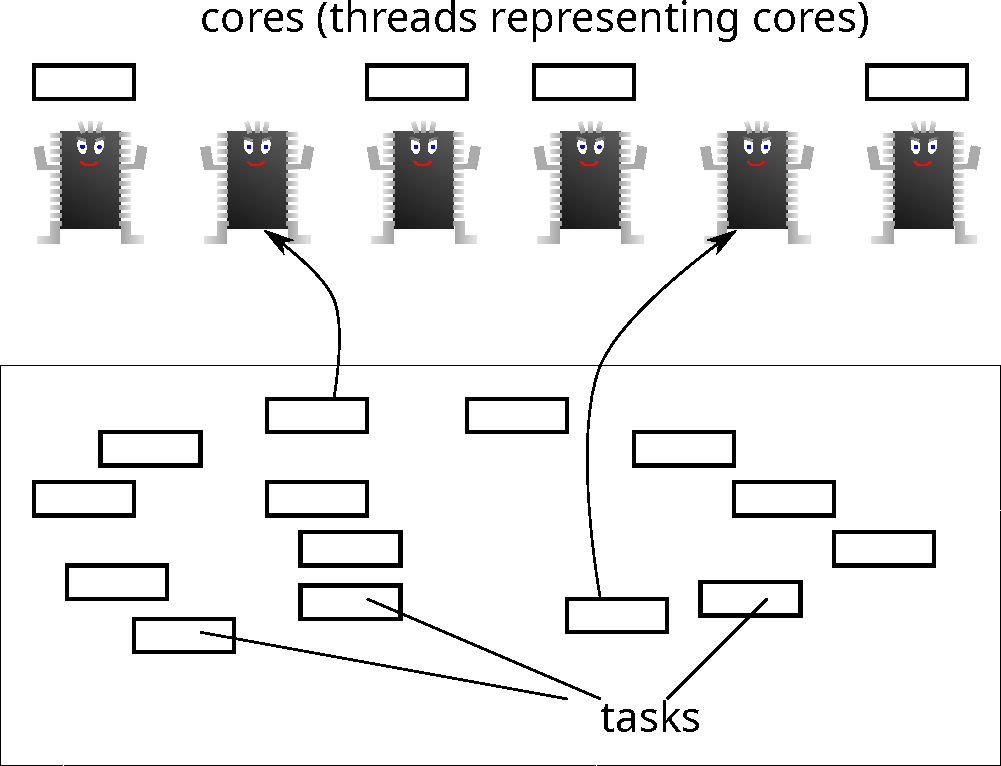
\includegraphics[width=\textwidth]{out/pdf/svg/tbb_approximated.pdf}  
\end{center}
\end{column}
\end{columns}
\end{frame}

%%%%%%%%%%%%%%%%% 
\begin{frame}[fragile]
\frametitle{A note on callable and C++ lambda expression}
\begin{itemize}
\item any {\em callable} object can be passed to {\tt run} method
\item a callable object is an object defining {\tt operator()}
\item e.g.
\begin{lstlisting}
class my_task {
  int x;
  my_task(int arg) { x = arg; }
  @\ao{void operator() ()}@ { print(x); }
}    
\end{lstlisting}
\begin{lstlisting}
tbb::task_group tg;
my_task c(3);
tg.run(c);
\end{lstlisting}
\end{itemize}
\end{frame}

%%%%%%%%%%%%%%%%% 
\begin{frame}
\frametitle{C++ lambda expression (closure)}
\begin{itemize}
\item it is cumbersome to manually define a class
  for each task creation; C++ lambda expression
  reduces this labor

  \begin{itemize}
  \item {\em not} specific to TBB, but a
    recent extension to C++ (C++0x, C++11) that
    TBB programmers would appreciate
  \end{itemize}

\item syntax in brief:
\begin{quote}
\ao{{\tt [}capture-list{\tt ] \{} statements {\tt \}}}
\end{quote}
this represents a callable object that, when called,
executes \ao{\em statements}.

\item \ao{\em capture-list} specifies which
  variables to {\em copy} into the
  closure, and which variables to {\em
    share} between the closure and the outer context

\end{itemize}
\end{frame}

%%%%%%%%%%%%%%%%% 
\begin{frame}[fragile]
\frametitle{C++ lambda expression examples (1)}
\begin{itemize}
\item copy everything ({\tt x} and {\tt y});
\begin{lstlisting}
int x = 3;
C = @\ao{[=]}@ { print(x); };
x = 4;
C(); // will print 3, not 4
\end{lstlisting}

\item share everything
\begin{lstlisting}
int x = 3;
C = @\ao{[\&]}@ { print(x); };
x = 4;
C(); // will print 4, not 3
\end{lstlisting}
\end{itemize}
\end{frame}


%%%%%%%%%%%%%%%%% 
\begin{frame}[fragile]
\frametitle{C++ lambda expression examples (2)}
\begin{itemize}
\item share specific variables
\begin{lstlisting}
int z;
C = [=,@\ao{\&z}@] { z = 4; };
C();
print(z); // will print 4, not 3
\end{lstlisting}

\item you will (often) 
  like to share large arrays to avoid large copies
\begin{lstlisting}
int a[1000];
C = [=,@\ao{\&a}@] { gemm(a) };
C();
\end{lstlisting}
\end{itemize}
\end{frame}

%%%%%%%%%%%%%%%%% 
\begin{frame}[fragile]
\frametitle{Which variables to share/copy when you {\tt run}?}
\begin{itemize}
\item if you want to get a return value, 
  do not forget to share the receiving variable 
  \begin{itemize}
  \item presumably wrong
\begin{lstlisting}
tg.run([=] { @\aka{\tt y}@ = f(x); });
\end{lstlisting}
  \item you should insead write:
\begin{lstlisting}
tg.run([=,@\ao{\tt \&y}@] { y = f(x); });
\end{lstlisting}
  \end{itemize}

\item make sure arguments you passed to the task 
  are not overwritten by the parent
  \begin{itemize}
  \item presumably wrong
\begin{lstlisting}
for (i = 0; i < n; i++) {
  tg.run([&] { y = f(@\aka{\tt i}@); });
}
\end{lstlisting}
  \item you should insead write:
\begin{lstlisting}
tg.run([&,@\ao{\tt =i}@] { y = f(i); });
\end{lstlisting}
  \end{itemize}
\end{itemize}
\end{frame}
\fi

%%%%%%%%%%%%%%%%%%%%%%%%%%%%%%%%%% 
\section{Reasoning about speedup}
%%%%%%%%%%%%%%%%%%%%%%%%%%%%%%%%%% 

%%%%%%%%%%%%%%%%% 
\begin{frame}
\frametitle{Reasoning about speedup}

\begin{itemize}

\item<1-> so you parallelized your program, you now
  hope to get some speedup on parallel machines!

\item<2-> \aka{PROBLEM:} how to reason about
  the execution time (thus speedup) of the program with $P$
  processors

\begin{center}

\includegraphics[width=0.2\textwidth]{out/pdf/svg/Question_Girl.pdf}  
\end{center}

\item<3-> \ao{ANSWER:} get the 
  \ao{\em work} and the \ao{\em critical path length} 
  of the computation
\end{itemize}
\end{frame}

%%%%%%%%%%%%%%%%%%%%%%%%%%%%%%%%%% 
\subsection{Work and critical path length}

%%%%%%%%%%%%%%%%% 
\iffalse
\begin{frame}[fragile]
\frametitle{Not \aka{\em parallelism}, but \ao{\em critical path}}

\begin{itemize}
\item What is {\em critical path}?
$\Rightarrow$ 
the longest \ao{\em dependent chain of computation}

\item Example (in a pseudo code):  
\begin{lstlisting}
main() {
  A();
  create_task(B());
  C();
  wait(); // wait for B
  D();
}    
\end{lstlisting}
\item Critical path is either 
  \begin{itemize}
  \item A() $\rightarrow$ B() $\rightarrow$ D()
  \item A() $\rightarrow$ C() $\rightarrow$ D()
  \end{itemize}
\end{itemize}
\end{frame}
\fi

%%%%%%%%%%%%%%%%% 
\begin{frame}[fragile]
\frametitle{Work and critical path length}
\begin{itemize}
\item \ao{\textbf{Work:}} $=$ the total amount of work of the computation
  \begin{itemize}
  \item $=$ the time it takes in a serial execution
  \end{itemize}

\item \ao{\textbf{Critical path length:}} 
  $=$ the maximum length of dependent chain of computation 
  \begin{itemize}
  \item a more precise definition follows, 
    with \ao{\em computational DAGs}
  \end{itemize}
\end{itemize}
\end{frame}


%%%%%%%%%%%%%%%%% 
\begin{frame}[fragile]
\frametitle{Computational DAGs}
\begin{columns}[t]
\begin{column}{0.65\textwidth}
\ao{\em The DAG} of a computation is a directed acyclic graph in which:
\begin{itemize}
\item a node $=$ an interval of computation 
free of task parallel primitives
% \begin{itemize}
% \item i.e. a node {\em starts} and {\em ends} 
%   by a task parallel primitive
% \item we assume a single node is executed non-preemptively
% \end{itemize}

\item an edge $=$ a dependency between two nodes, of three types:
  \begin{itemize}
  \item parent $\rightarrow$ created child
  \item child $\rightarrow$ waiting parent
  \item a node $\rightarrow$ the next node in the same task
  \end{itemize}
\end{itemize}
\end{column}

\begin{column}{0.30\textwidth}
\begin{lstlisting}
main() {
  A();
  create task for B();
  C();
  wait(); // wait for B
  D();
}    
\end{lstlisting}

\begin{center}
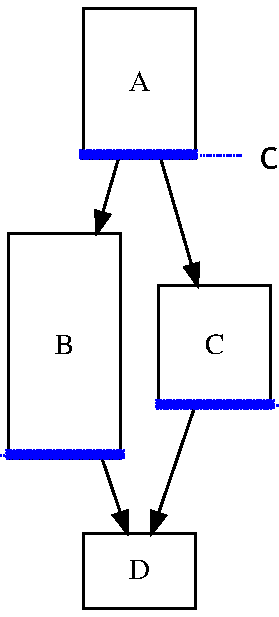
\includegraphics[width=\textwidth]{out/pdf/svg/dag.pdf}
\end{center}
\end{column}
\end{columns}
\end{frame}

%%%%%%%%%%%%%%%%% 
\begin{frame}[fragile]
\frametitle{A computational DAG and critical path length}
\begin{columns}[t]
\begin{column}{0.65\textwidth}
\begin{itemize}
\item Consider each node is augmented with the time
  it takes for a processor to execute it (\ao{\em the node's execution time})

\item Define {\em the length of a path} to be the
  sum of execution time of the nodes on the path
\end{itemize}

\end{column}

\begin{column}{0.35\textwidth}
\begin{center}
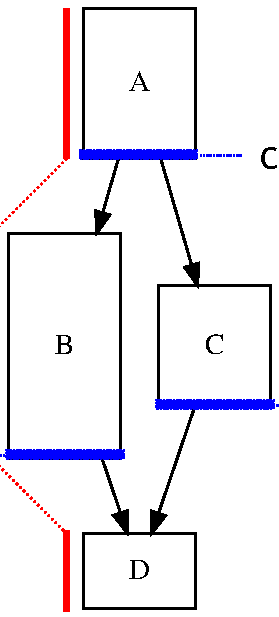
\includegraphics[width=\textwidth]{out/pdf/svg/dag_cp.pdf}
\end{center}
\end{column}
\end{columns}

Given a computational DAG,
\begin{quote}
\ao{critical path length 
  = the length of the longest 
  path from the start node to the end node in the DAG}
\end{quote}

(we often say {\em critical path} to in fact mean its length)
\end{frame}



%%%%%%%%%%%%%%%%% 
\begin{frame}[fragile]
\frametitle{A computational DAG and work}
\begin{columns}[t]
\begin{column}{0.65\textwidth}
\begin{itemize}
\item Work, too, can be elegantly defined in light of computational DAGs
\end{itemize}
\end{column}

\begin{column}{0.35\textwidth}
\begin{center}
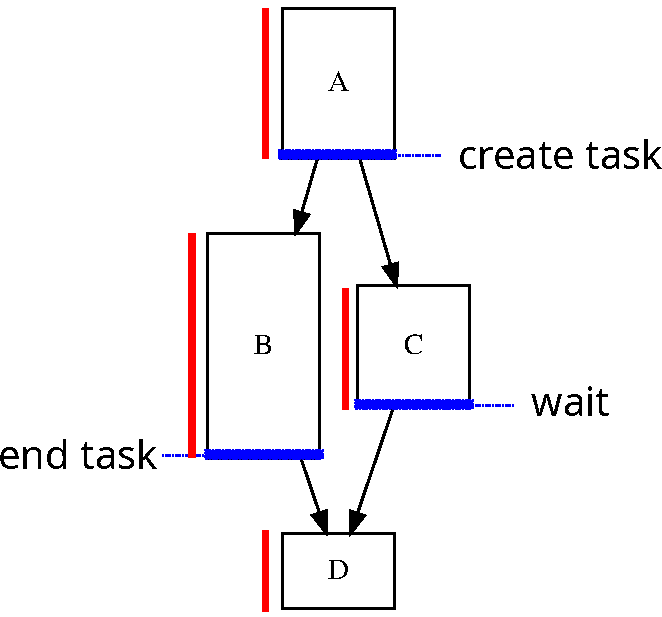
\includegraphics[width=\textwidth]{out/pdf/svg/dag_work.pdf}
\end{center}
\end{column}
\end{columns}

Given a computational DAG,
\begin{quote}
\ao{work = the sum of lengths of all nodes}
\end{quote}

\end{frame}


%%%%%%%%%%%%%%%%% 
\begin{frame}[fragile]
\frametitle{What do they intuitively mean?}
\begin{columns}
\begin{column}{0.7\textwidth}
\begin{itemize}
\item The critical path length represents 
  the ``ideal'' execution time with 
  {\em infinitely many} processors
  \begin{itemize}
  \item i.e., each node is executed immediately after
    all its predecessors have finished
  \end{itemize}

\item We thus often denote it by \ao{$T_\infty$}

\item Analogously, we often denote \ao{\em work} by \ao{$T_1$}
\end{itemize}

\begin{quote}
\ao{$T_1 = $ work, $T_\infty = $ critical path}
\end{quote}
\end{column}

\begin{column}{0.3\textwidth}
\begin{center}
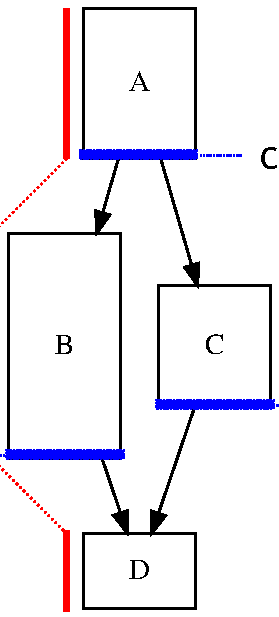
\includegraphics[width=\textwidth]{out/pdf/svg/dag_cp.pdf}

\vskip-2mm

{\footnotesize critical path length}

\vskip3mm

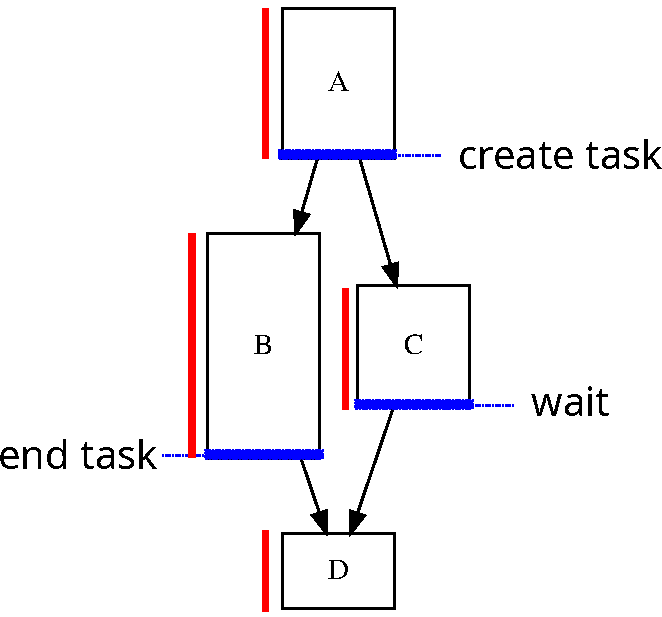
\includegraphics[width=\textwidth]{out/pdf/svg/dag_work.pdf}

\vskip-2mm

{\footnotesize work}
\end{center}
\end{column}
\end{columns}

\end{frame}


%%%%%%%%%%%%%%%%% 
\begin{frame}
\frametitle{Why are they important?}

\begin{itemize}
\item<1-> Now you understood what the critical path is

\item<2-> But why is it a good tool to
  understand speedup?

\begin{center}

\includegraphics[width=0.2\textwidth]{out/pdf/svg/Question_Girl.pdf}  
\end{center}

\item<3-> \aka{QUESTION:} Specifically, what does it tell us about 
  performance or speedup on, say, my 64 core machines?

\item<4-> \ao{ANSWER:} A beautiful theorem 
  (\ao{\em greedy scheduler theorem}) gives us an answer
\end{itemize}
\end{frame}


%%%%%%%%%%%%%%%%%%%%%%%%%%%%%%%%%% 
\subsection{Greedy scheduler theorem}
%%%%%%%%%%%%%%%%% 
\begin{frame}
\frametitle{The greedy scheduler theorem}

\begin{itemize}
\item<1-> Assume:
  \begin{itemize}
  \item you have $P$ processors
  \item they are \ao{\em greedy}, in the sense that 
    a processor is \ao{\em always busy} on a node whenever 
    there is \ao{\em any runnable} node (a node whose predecessors have finished) in the entire system
  \item an execution time of a node does not depend on
    which processor executed it
  \end{itemize}

\item<2-> Theorem: 
  given a computational DAG of:
  \begin{itemize}
  \item work $T_1$ and
  \item critical path $T_\infty$,
  \end{itemize}
  the execution time 
  with $P$ processors, \ao{$T_P$}, satisfies
  \[ \ao{T_P \leq \frac{T_1 - T_\infty}{P} + T_\infty} \]

\item<3-> in practice you remember a simpler form:
  \[ \ao{T_P \leq \frac{T_1}{P} + T_\infty} \]
\end{itemize}
\end{frame}


%%%%%%%%%%%%%%%%% 
\begin{frame}
\frametitle{The greedy scheduler theorem}
\begin{itemize}
\item it is now a common sense in parallel computing, but
the root of the idea seems:

\begin{quote}
{\em Richard Brent.}
The Parallel Evaluation of General Arithmetic Expressions.
{\em Journal of the ACM 21(2). pp201-206. 1974}
\end{quote}

\begin{quote}
{\em Derek Eager, John Zahorjan, and Edward Lazowska.}
  Speedup versus efficiency in parallel systems.
{\em IEEE Transactions on Computers 38(3). pp408-423. 1989}
\end{quote}

\item People attribute it to Brent and call it 
  \ao{Brent's theorem}

\item Proof is a good exercise for you
\end{itemize}
\end{frame}

%%%%%%%%%%%%%%%%% 
\begin{frame}
\frametitle{I'll repeat! Remember it!}


{\huge \[ \ao{T_P \leq \frac{T_1}{P} + T_\infty} \]}

\end{frame}


%%%%%%%%%%%%%%%%% 
\begin{frame}
\frametitle{A few facts that help you understand it}
Consider the execution time with $P$ processors ($T_P$)
\begin{itemize}
\item there are two obvious {\it lower bounds}
  \begin{itemize}
  \item \ao{$T_P \geq \frac{T_1}{P}$}
  \item \ao{$T_P \geq T_\infty$}
  \end{itemize}
  or more simply,
\[ \ao{T_P \geq \max\left(\frac{T_1}{P}, T_\infty\right)} \]

\item what a greedy scheduler achieves is
  \[ \ao{T_P \leq \mbox{sum}\left(\frac{T_1}{P}, T_\infty\right)} \]
\item two memorable facts
  \begin{itemize}
  \item {\it ``the sum of two lower bounds is an upper bound''}
  \item any greedy scheduler is
    within a factor of two of the optimal scheduler
    (下手な考え休むに似たり?)
  \end{itemize}
\end{itemize}
\end{frame}

%%%%%%%%%%%%%%%%% 
\begin{frame}
\frametitle{A few facts to remember about $T_1$ and $T_\infty$}
\begin{itemize}
\item to get good (nearly perfect) speedup, we wish to have
  \[ \frac{T_1}{P} \gg T_\infty \]
  or equivalently, 
  \[ \frac{T_1}{T_\infty} \gg P \]

\item we can consider $\frac{T_1}{T_\infty}$
  to be {\it the average parallelism} (the speedup we would get
  with infinitely many processors)

\item we like to make the average parallelism
  large enough compared to the actual number of processors

\end{itemize}
\end{frame}

%%%%%%%%%%%%%%%%% 
\begin{frame}
\frametitle{Takeaway message}

\begin{quote}
{\Large Suffer from low speedup?
$\Rightarrow$
\ao{try to shorten the critical path}}
\end{quote}

{\small
\begin{quote}
people are tempted to think
creating \aka{more and more tasks} is the way; 
they are useless, unless it shortens the 
critical path
\end{quote}}

\begin{center}
\def\svgwidth{0.6\textwidth}
{\scriptsize \input{out/tex/svg/why_cp3.pdf_tex}}
\end{center}
\end{frame}

%%%%%%%%%%%%%%%%% 
\begin{frame}
  \frametitle{A special case (1) --- Amdahl's law}
  \begin{itemize}
  \item assume the entire computation ($T_1$)
    consists of two parts,
    \begin{enumerate}
    \item one completely serial
      ($T_\infty$), and
    \item the other completely parallelizable
      ($T_1 - T_\infty$)
    \end{enumerate}
  \begin{center}
    \def\svgwidth{0.7\columnwidth}
    {\scriptsize\input{out/tex/svg/amdahl.pdf_tex}}
  \end{center}
  \item Amdahl's law states $T_p \geq T_\infty$, which is trivial
  \item it is also trivial to observe that {\it any} greedy scheduler achieves
    \[ T_P \leq \frac{T_1 - T_\infty}{P} + T_\infty, \]
    which coincides with what the greedy scheduler theorem says
    (for more general cases)
  \item takeaway: want to get a good speedup? $\Rightarrow$ minimize $T_\infty$, or the work not parallelized
  \end{itemize}
\end{frame}

%%%%%%%%%%%%%%%%% 
\begin{frame}
  \frametitle{A special case (2) --- ``bag of tasks''}
  \begin{itemize}
  \item assume we have a set of $n$ indepedent tasks whose runtimes are
    $t_1, t_2, \cdots , t_n$

    \begin{center}
      \def\svgwidth{0.5\columnwidth}
      \input{out/tex/svg/bag_of_tasks.pdf_tex}  
\end{center}

  \item consider a dynamic greedy scheduler in which each core repeats
    fetching a task at a time and executing it
  \item then
    \begin{itemize}
    \item $T_1 = t_1 + t_2 + \cdots + t_n$
    \item $T_\infty = \max(t_1, t_2, \cdots , t_n)$
    \end{itemize}
  \item takeaway : you want to get a good speedup? $\Rightarrow$ shorten
    $\max(t_1, t_2, \cdots , t_n)$,
    or the execution time of the \ao{\it longest} task
  \end{itemize}

\end{frame}

%%%%%%%%%%%%%%%%% 
\begin{frame}
\frametitle{What makes $T_\infty$ so useful?}
$T_\infty$ is:
\begin{itemize}
\item a single \ao{\em global metric} (just as the work is)
  \begin{itemize}
  \item not something that fluctuates over time
    (cf. the number of tasks)
  \end{itemize}

\item \ao{\em inherent to the algorithm,
    independent from the scheduler}
  \begin{itemize}
  \item not something that depends on schedulers
  \end{itemize}

\item connected to execution time with $P$
  processors in a beautiful way (\ao{$T_P \leq T_1/P
  + T_\infty$})

\item \ao{easy to estimate/calculate}
  (like the ordinary time complexity of serial programs, as we will see below)
\end{itemize}

\end{frame}

%%%%%%%%%%%%%%%%%%%%%%%%%%%%%%%%%% 
\subsection{Calculating work and critical path}
%%%%%%%%%%%%%%%%% 
\begin{frame}[fragile]
\frametitle{Calculating work and critical
  path}

\begin{itemize}
\item for recursive procedures, 
  using recurrent equations is often a good
  strategy
\item e.g., if we have
  \begin{columns}
    \begin{column}{0.6\textwidth}
\begin{lstlisting}
f(n) {
  if (n == 1) { trivial(n); /* assume O(1) */ }
  else {
    g(n);
    create_task f(n/3);
    f(2*n/3);
    wait();
  }
}    
\end{lstlisting}
    \end{column}
    \begin{column}{0.3\textwidth}
\begin{center}
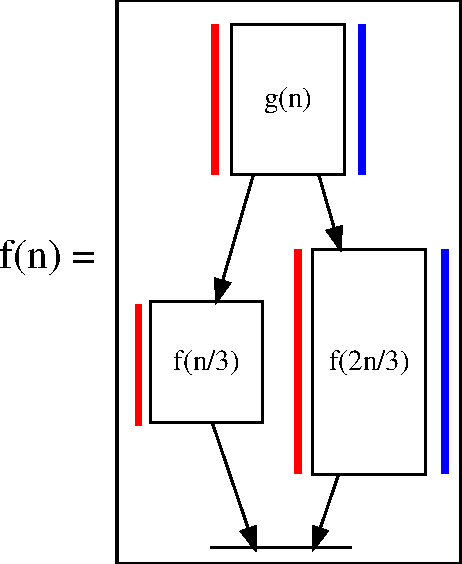
\includegraphics[width=\textwidth]{out/pdf/svg/dag_f.pdf}  
\end{center}
    \end{column}
  \end{columns}
then
\begin{itemize}
\item (work)
\aka{$W_{\mbox{f}}(n) \leq W_{\mbox{g}}(n) + W_{\mbox{f}}(n/3) + W_{\mbox{f}}(2n/3)$}
\item (critical path)
\ao{$C_{\mbox{f}}(n) \leq C_{\mbox{g}}(n) + \max \{ C_{\mbox{f}}(n/3), C_{\mbox{f}}(2n/3) \}$}
\end{itemize}

\item we apply this for programs we have seen
\end{itemize}
\end{frame}


%%%%%%%%%%%%%%%%% 
\begin{frame}[fragile]
\frametitle{Work of $k$-d tree construction}
\begin{itemize}
\item []
\begin{lstlisting}
build(P, R, depth) {
  if (|P| == 0) {
    return 0; /* empty */
  } else if (|P| <= threshold) {
    return make_leaf(P, R, depth);
  } else {
    p = find_pivot(P, depth % D);
    R0,R1 = split_rect(R, depth % D, p.pos[depth % D]);
    P0,P1 = partition(P - { p }, depth % D, p.pos[depth % D]);
    n0 = @\ao{\tt create\_task build}@(P0, R0, depth + 1);
    n1 = @\ao{\tt build}@(P1, R1, depth + 1);
    wait();
    return make_node(p, n0, n1, depth);
  } }
\end{lstlisting}

\item []
  recall that {\tt partition}
  takes time proportional to $n$ (the number of points). thus, 
\[
\begin{array}{l}
W_{\mbox{\scriptsize build}}(n)
\approx 2W_{\mbox{\scriptsize build}}(n/2) + \Theta(n) \\
\end{array}
\]

\item [] omitting math,
\[ \therefore W_{\mbox{\scriptsize build}}(n) \in \ao{\Theta(n \log n)} \]
\end{itemize}
\end{frame}

%%%%%%%%%%%%%%%%% 
\begin{frame}
\frametitle{Remark}
\begin{itemize}
\item the argument above is crude and optimistic, as $n$
  points are not always split into two sets of
  equal sizes

\item omitting math again, the $\Theta(n \log n)$ result is valid as
  long as a split is guaranteed to be ``never too
  unbalanced'' (i.e., there is a constant $\alpha
  < $, s.t. each child gets $\leq \alpha n$
  points)
\end{itemize}
\end{frame}

%%%%%%%%%%%%%%%%% 
\begin{frame}[fragile]
\frametitle{Critical path}
\begin{itemize}
\item []
\begin{lstlisting}
@\ao{\tt build}@(P, R, depth) {
  if (|P| == 0) {
    return 0; /* empty */
  } else if (|P| <= threshold) {
    return make_leaf(P, R, depth);
  } else {
    p = find_pivot(P, depth % D);
    R0,R1 = split_rect(R, depth % D, p.pos[depth % D]);
    P0,P1 = partition(P - { p }, depth % D, p.pos[depth % D]);
    n0 = @\ao{\tt create\_task build}@(P0, R0, depth + 1);
    n1 = @\ao{\tt build}@(P1, R1, depth + 1);
    wait();
    return make_node(p, n0, n1, depth);
  } }
\end{lstlisting}

\item []
\[
\begin{array}{l}
C_{\mbox{\scriptsize build}}(n)
\approx C_{\mbox{\scriptsize build}}(n/2) + \Theta(n) \\
\end{array}
\]
\item [] omitting math,
\[ \therefore C_{\mbox{\scriptsize build}}(n) \in \ao{\Theta(n)} \]
\end{itemize}
\end{frame}


%%%%%%%%%%%%%%%%% 
\begin{frame}
\frametitle{Speedup of $k$-d tree construction}
\begin{itemize}
\item Now we have:
\[ 
\begin{array}{l}
W_{\mbox{\scriptsize build}}(n) \in \Theta(n\log n), \\
C_{\mbox{\scriptsize build}}(n) \in \Theta(n).
\end{array}
\]

\item $\Rightarrow$ 
\[ \frac{T_1}{T_\infty} \in \Theta(\log n) \]

\item not satisfactory in practice
\end{itemize}
\end{frame}

%%%%%%%%%%%%%%%%% 
\begin{frame}
\frametitle{What the analysis tells us}
\begin{itemize}
\item the expected speedup, \ao{$\Theta(\log n)$}, is not satisfactory
\item to improve, shorten its critical path \ao{$\Theta(n)$}, to \ao{$o(n)$}
\item where you should improve? the reason for the $\Theta(n)$ critical path
  is \ao{\texttt{partition}}; we should parallelize \ao{\texttt{partition}}
%\item this is left to the hands-on session 
%  (hint: divide and conquer thinking)
\end{itemize}

\begin{center}
\def\svgwidth{0.7\textwidth}
\input{out/tex/svg/kdtree_partition.pdf_tex}
\end{center}


\end{frame}


\section{More divide and conquer examples}
%%%%%%%%%%%%%%%%%%%%%%%%%%%%%%%%%% 

%%%%%%%%%%%%%%%%%
\iffalse
\begin{frame}
\frametitle{Two more divide and conquer examples}
\begin{itemize}
\item Merge sort
\item Cholesky factorization and its component matrix problems
\end{itemize}
\end{frame}
\fi

%%%%%%%%%%%%%%%%%%%%%%%%%%%%%%%%%% 
\subsection{Merge sort}
%%%%%%%%%%%%%%%%%%%%%%%%%%%%%%%%%% 

%%%%%%%%%%%%%%%%% 
\begin{frame}
\frametitle{Merge sort}
\begin{itemize}
\item Input: 
  \begin{itemize}
  \item \ao{$A$}: an array
  \end{itemize}
\item Output:
  \begin{itemize}
  \item \ao{$B$}: a sorted array
  \end{itemize}
\item Note: the result could be returned either in place
  or in a separate array. Assume it is ``in place'' in the following.
\end{itemize}
\end{frame}

%%%%%%%%%%%%%%%%% 
\begin{frame}[fragile]
\frametitle{Merge sort : serial code}
\begin{columns}
\begin{column}{0.45\textwidth}
\begin{lstlisting}
/* sort a..a_end and put the result into
   (i)  a (if dest = 0)
   (ii) t (if dest = 1) */
void @\ao{\tt ms}@(elem * a, elem * a_end, 
        elem * t, int dest) {
  long n = a_end - a;
  if (n == 1) {
    if (dest) t[0] = a[0];
  } else {
    /* split the array into two */
    long nh = n / 2;
    elem * c = a + nh;
    /* sort 1st half */
    @\ao{\tt ms}@(a, c,     t,      1 - dest);
    /* sort 2nd half */
    @\ao{\tt ms}@(c, a_end, t + nh, 1 - dest);
    elem * s = (dest ? a : t);
    elem * d = (dest ? t : a);
    /* merge them */
    @\mura{\tt merge}@(s,      s + nh, 
          s + nh, s + n, d);
  }
}
\end{lstlisting}
\end{column}

\begin{column}{0.43\textwidth}
\begin{lstlisting}
/* merge a_beg ... a_end 
     and b_beg ... b_end 
    into c */
void 
@\mura{merge}@(elem * a, elem * a_end, 
      elem * b, elem * b_end, 
      elem * c) {
  elem * p = a, * q = b, * r = c;
  while (p < a_end && q < b_end) {
    if (*p < *q) { *r++ = *p++; }
    else { *r++ = *q++; }
  }
  while (p < a_end) *r++ = *p++;
  while (q < b_end) *r++ = *q++;
}
\end{lstlisting}

\aka{note:} as always, actually switch to serial sort below a threshold
  (not shown in the code above)
\end{column}
\end{columns}
\end{frame}

%%%%%%%%%%%%%%%%% 
\begin{frame}[fragile]
\frametitle{Merge sort : parallelization}
\begin{columns}
\begin{column}{0.6\textwidth}
\begin{lstlisting}
void @\ao{\tt ms}@(elem * a, elem * a_end, 
        elem * t, int dest) {
  long n = a_end - a;
  if (n == 1) {
    if (dest) t[0] = a[0];
  } else {
    /* split the array into two */
    long nh = n / 2;
    elem * c = a + nh;
    /* sort 1st half */
    @\ao{\tt create\_task ms}@(a, c,     t,      1 - dest);
    /* sort 2nd half */
    @\ao{\tt ms}@(c, a_end, t + nh, 1 - dest);
    @\ao{\tt wait()}@;
    elem * s = (dest ? a : t);
    elem * d = (dest ? t : a);
    /* merge them */
    @\mura{\tt merge}@(s,      s + nh, 
          s + nh, s + n, d);
  }
}
\end{lstlisting}
\end{column}

\begin{column}{0.4\textwidth}
\begin{itemize}
\item Will we get ``good enough'' speedup?
\end{itemize}
\end{column}

\end{columns}
\end{frame}

\iffalse
%%%%%%%%%%%%%%%%% 
\begin{frame}
\frametitle{Empirically, we don't \ldots}

\begin{itemize}
\item Remember this?
  \begin{itemize}
  \item Critical path limit:
    \[ T_P \geq T_\infty \]
  \item Greedy scheduler theorem:
    \[ T_P \leq \frac{T_1}{P} + T_\infty \]
  \end{itemize}
\item $\Rightarrow$ analyze its $T_1$ and $T_\infty$
\end{itemize}
\end{frame}
\fi

%%%%%%%%%%%%%%%%% 
\begin{frame}[fragile]
\frametitle{Work of merge sort}
\begin{columns}
\begin{column}{0.48\textwidth}
\begin{lstlisting}
void @\ao{\tt ms}@(elem * a, elem * a_end, 
        elem * t, int dest) {
  long n = a_end - a;
  if (n == 1) {
    if (dest) t[0] = a[0];
  } else {
    /* split the array into two */
    long nh = n / 2;
    elem * c = a + nh;
    /* sort 1st half */
    @\ao{\tt create\_task ms}@(a, c, t, 1 - dest);
    /* sort 2nd half */
    @\ao{\tt ms}@(c, a_end, t + nh, 1 - dest);
    @\ao{\tt wait()}@;
    elem * s = (dest ? a : t);
    elem * d = (dest ? t : a);
    /* merge them */
    @\mura{\tt merge}@(s,      s + nh, 
          s + nh, s + n, d);
  }
}
\end{lstlisting}
\end{column}

\begin{column}{0.52\textwidth}
\[
\begin{array}{l}
W_{\mbox{\scriptsize ms}}(n)
= 2W_{\mbox{\scriptsize ms}}(n/2)
+ W_{\mbox{\scriptsize merge}}(n), \\
W_{\mbox{\scriptsize merge}}(n) \in \Theta(n).
\end{array}
\]

\[ \therefore W_{\mbox{\scriptsize ms}}(n) \in \ao{\Theta(n \log n)} \]
\end{column}
\end{columns}
\end{frame}

%%%%%%%%%%%%%%%%% 
\begin{frame}[fragile]
\frametitle{Critical path of merge sort}

\begin{columns}
\begin{column}{0.48\textwidth}
\begin{lstlisting}
void @\ao{\tt ms}@(elem * a, elem * a_end, 
        elem * t, int dest) {
  long n = a_end - a;
  if (n == 1) {
    if (dest) t[0] = a[0];
  } else {
    /* split the array into two */
    long nh = n / 2;
    elem * c = a + nh;
    /* sort 1st half */
    @\ao{\tt create\_task ms}@(a, c, t, 1 - dest);
    /* sort 2nd half */
    @\ao{\tt ms}@(c, a_end, t + nh, 1 - dest);
    @\ao{\tt wait()}@;
    elem * s = (dest ? a : t);
    elem * d = (dest ? t : a);
    /* merge them */
    @\mura{\tt merge}@(s,      s + nh, 
          s + nh, s + n, d);
  }
}
\end{lstlisting}
\end{column}

\begin{column}{0.52\textwidth}
\[ 
\begin{array}{l}
C_{\mbox{\scriptsize ms}}(n)
= C_{\mbox{\scriptsize ms}}(n/2)
+ C_{\mbox{\scriptsize merge}}(n), \\
C_{\mbox{\scriptsize merge}}(n) \in \Theta(n)
\end{array}
\]

\[ \therefore C_{\mbox{\scriptsize ms}}(n) \in \ao{\Theta(n)} \]
\end{column}
\end{columns}
\end{frame}

%%%%%%%%%%%%%%%%% 
\begin{frame}
\frametitle{Speedup of merge sort}
\[ 
\begin{array}{l}
T_1 = W_{\mbox{\scriptsize ms}}(n) \in \Theta(n\log n), \\
T_\infty = C_{\mbox{\scriptsize ms}}(n) \in \Theta(n).
\end{array}
\]
the average parallelism
\[ T_1/T_\infty \in \Theta(\log n). \]
\end{frame}

%%%%%%%%%%%%%%%%%
\iffalse
\begin{frame}
\frametitle{Visualizing parallelism}
\begin{itemize}
\item Clearly, the ``the last merge step''
  causes $\Theta(n)$ serial work
\item We must have a parallel merge with $o(n)$ critical path
\end{itemize}
\end{frame}
\fi

%%%%%%%%%%%%%%%%% 
\begin{frame}[fragile]
\frametitle{How (serial) merge works}
\begin{columns}
\begin{column}{0.5\textwidth}
\begin{lstlisting}
/* merge a_beg ... a_end 
     and b_beg ... b_end 
    into c */
void 
@\mura{merge}@(elem * a, elem * a_end, 
      elem * b, elem * b_end, 
      elem * c) {
  elem * p = a, * q = b, * r = c;
  while (p < a_end && q < b_end) {
    if (*p < *q) { *r++ = *p++; }
    else { *r++ = *q++; }
  }
  while (p < a_end) *r++ = *p++;
  while (q < b_end) *r++ = *q++;
}
\end{lstlisting}
\end{column}

\begin{column}{0.5\textwidth}
\begin{center}
\def\svgwidth{\columnwidth}
\only<1>{\scriptsize \input{out/tex/svg/merge1.pdf_tex}}
\only<2>{\scriptsize \input{out/tex/svg/merge2.pdf_tex}}
\only<3>{\scriptsize \input{out/tex/svg/merge3.pdf_tex}}
\end{center}
\end{column}
\end{columns}
Looks very serial \ldots
\end{frame}


%%%%%%%%%%%%%%%%% 
\begin{frame}
\frametitle{How to parallelize merge?}
\begin{itemize}
\item again, divide and conquer thinking helps
\item left as an exercise
\end{itemize}
\end{frame}

%%%%%%%%%%%%%%%%%%%%%%%%%%%%%%%%%% 
\subsection{Cholesky factorization}
%%%%%%%%%%%%%%%%% 
\begin{frame}
\frametitle{Our running example : Cholesky factorization}
\begin{itemize}
\item Input: 
  \begin{itemize}
  \item \ao{$A$}: $n\times n$ positive semidefinite symmetric matrix
  \end{itemize}
\item Output: 
  \begin{itemize}
  \item \aka{$L$}: $n\times n$ lower triangular matrix s.t.
\[ \ao{A} = \aka{L \; {}^tL} \]
  \item (${}^t L$ is a transpose of $L$)
  \end{itemize}
\end{itemize}

\begin{figure}
\centering
\def\svgwidth{0.8\textwidth}
{\input{out/tex/svg/chol.pdf_tex}}
\end{figure}

\end{frame}


%%%%%%%%%%%%%%%%% 
\begin{frame}
\frametitle{Note : why Cholesky factorization is important?}
\begin{itemize}
\item It is the core step when solving
\[ Ax = b \quad \mbox{(single righthand side)} \]
or, in more general,
\[ AX = B \quad \mbox{(multiple righthand sides)}, \]
as follows.
\begin{enumerate}
\item Cholesky decompose $A = L \; {}^tL$ and get
\[ 
\begin{array}{cccc}
L & \underbrace{{}^tL X} & = & B \\
  & Y                    &   &   \\
\end{array}
\]
\item Find $X$ by solving triangular systems twice
  \begin{enumerate}
  \item $L Y = B$
  \item ${}^tL X = Y$
  \end{enumerate}
\end{enumerate}
\end{itemize}
\end{frame}

%%%%%%%%%%%%%%%%% 
\begin{frame}
\frametitle{Formulate using subproblems}

\[
\left(
\begin{array}{cc}
A_{11}     & {}^tA_{21} \\
A_{21}     & A_{22} \\
\end{array}
\right)
=
\left(
\begin{array}{cc}
L_{11}     & O     \\
L_{21} & L_{22} \\
\end{array}
\right)
\left(
\begin{array}{cc}
{}^tL_{11} & {}^tL_{21} \\
O         & {}^tL_{22} \\
\end{array}
\right)
\]
leads to three subproblems
\begin{enumerate}
\item $A_{11} = L_{11} \; {}^tL_{11}$
\item ${}^tA_{21} = L_{11} \; {}^tL_{21}$
\item $A_{22} = L_{21}\; {}^tL_{21} + L_{22} \; {}^tL_{22}$
\end{enumerate}

%\def\svgwidth{\textwidth}
%{\input{out/tex/svg/lu.pdf_tex}}

\end{frame}

%%%%%%%%%%%%%%%%% 
\begin{frame}[fragile]
\frametitle{Solving with recursions}

\[
\left(
\begin{array}{cc}
A_{11} & {}^tA_{21} \\
A_{21} & A_{22} \\
\end{array}
\right)
=
\left(
\begin{array}{cc}
L_{11}     & O     \\
L_{21} & L_{22} \\
\end{array}
\right)
\left(
\begin{array}{cc}
{}^tL_{11} & {}^tL_{21} \\
O         & {}^tL_{22} \\
\end{array}
\right)
\]


\begin{columns}[t]
\begin{column}{0.53\textwidth}
\begin{enumerate}
\item $A_{11} = L_{11} \; {}^tL_{11}$ \\
  \begin{itemize}
  \item<2-> recursion and get $\aka{L_{11}}$
  \end{itemize}
\item ${}^tA_{21} = \aka{L_{11}}  \; {}^tL_{21}$ \\
  \begin{itemize}
  \item<3-> solve a {\em triangular} system and get $\aka{{}^tL_{21}}$
  \end{itemize}
\item$A_{22} = \aka{L_{21}{}^tL_{21}} + L_{22} \; {}^tL_{22}$ \\
  \begin{itemize}
  \item<4->
    recursion on $(A_{22} - \aka{L_{21}{}^tL_{21}})$ and get $\aka{L_{22}}$
  \end{itemize}
  % \item If $n = 1$, the problem is trivial $l_{11} = \sqrt{a_{11}}$
\end{enumerate}
\end{column}

\begin{column}{0.45\textwidth}
\begin{lstlisting}[basicstyle=\scriptsize]
/* Cholesky factorization */
chol(@$A$@) {
  if (@$n$@ = 1) return (@$\sqrt{a_{11}}$@);
  else {
    @$L_{11}$@ = chol(@$A_{11}$@);
    /* triangular solve */
    @${}^tL_{21}$@ = trsm(@$L_{11}, {}^tA_{21}$@);
    @$L_{22}$@ = chol(@$A_{22} - L_{21}{}^tL_{21}$@);
    return @$\left(\begin{array}{cc} L_{11} & {}^tL_{21} \\ L_{21} & L_{22} \end{array}\right)$@
  }
}
\end{lstlisting}
\end{column}
\end{columns}
\end{frame}

%%%%%%%%%%%%%%%%% 
\begin{frame}[fragile]
\frametitle{Remark 1 : ``In-place update'' version}
\begin{itemize}
\item Instead of returning the answer as another matrix,
it is often possible to update the input matrix with the answer
\item When possible, it is desirable, as it avoids extra copies
\end{itemize}

\begin{columns}[t]
\begin{column}{0.5\textwidth}
\begin{lstlisting}[basicstyle=\scriptsize]
/* functional */
chol(@$A$@) {
  if (@$n$@ = 1) return (@$\sqrt{a_{11}}$@);
  else {
    @$L_{11}$@ = chol(@$A_{11}$@);
    /* triangular solve */
    @${}^tL_{21}$@ = trsm(@$L_{11}, {}^tA_{21}$@);
    @$L_{22}$@ = chol(@$A_{22} - L_{21}{}^tL_{21}$@);
    return @$\left(\begin{array}{cc} L_{11} & {}^tL_{21} \\ L_{21} & L_{22} \end{array}\right)$@
  }
}
\end{lstlisting}
\end{column}

\begin{column}{0.5\textwidth}
\begin{lstlisting}[basicstyle=\scriptsize]
/* in place */
chol(@$A$@) {
  if (@$n$@ = 1) @$a_{11} := \sqrt{a_{11}}$@;
  else {
    chol(@$A_{11}$@);
    /* triangular solve */
    trsm(@$A_{11}, A_{12}$@);
    @$A_{21} = {}^tA_{12}$@;
    @$A_{22} \minusequal A_{21} A_{12}$@
    chol(@$A_{22}$@);
  }
}
\end{lstlisting}
\end{column}
\end{columns}
\end{frame}

%%%%%%%%%%%%%%%%% 
\begin{frame}[fragile]
\frametitle{In-place Cholesky at work}

\begin{columns}[t]
\begin{column}{0.4\textwidth}
\begin{lstlisting}[basicstyle=\scriptsize]
/* in place */
chol(@$A$@) {
  if (@$n$@ = 1) @$a_{11} := \sqrt{a_{11}}$@;
  else {
    chol(@$A_{11}$@);
    /* triangular solve */
    trsm(@$A_{11}, A_{12}$@);
    @$A_{21} = {}^tA_{12}$@;
    @$A_{22} \minusequal A_{21} A_{12}$@
    chol(@$A_{22}$@);
  }
}
\end{lstlisting}
\end{column}
\begin{column}{0.6\textwidth}
\begin{center}
\def\svgwidth{\textwidth}
\only<1>{\input{out/tex/svg/chol_at_work_1.pdf_tex}}%
\only<2>{\input{out/tex/svg/chol_at_work_2.pdf_tex}}%
\only<3>{\input{out/tex/svg/chol_at_work_3.pdf_tex}}%
\only<4>{\input{out/tex/svg/chol_at_work_4.pdf_tex}}%
\only<5>{\input{out/tex/svg/chol_at_work_5.pdf_tex}}%
\only<6>{\input{out/tex/svg/chol_at_work_6.pdf_tex}}
\end{center}
\end{column}
\end{columns}
\end{frame}


%%%%%%%%%%%%%%%%% 
\begin{frame}[fragile]
\frametitle{Remark 2 : where to decompose}
\begin{itemize}
\item Where to partition $A$ is {\em arbitrary}
\item The case $n_1 = 1$ and $n_2 = n - 1$ $\approx$ loops
\end{itemize}

\begin{center}
\def\svgwidth{0.5\textwidth}
{\tiny\input{out/tex/svg/chol_decomp.pdf_tex}}
\end{center}

\begin{columns}[t]
\begin{column}{0.5\textwidth}
\begin{lstlisting}[basicstyle=\scriptsize]
/* general */
chol(@$A$@) {
  if (@$n$@ = 1) @$a_{11} := \sqrt{a_{11}}$@;
  else {
    chol(@$A_{11}$@);
    /* triangular solve */
    trsm(@$A_{11}, A_{12}$@);
    @$A_{21} = {}^tA_{12}$@;
    @$A_{22} \minusequal A_{21} A_{12}$@
    chol(@$A_{22}$@);
  }
}
\end{lstlisting}
\end{column}

\begin{column}{0.5\textwidth}
\begin{lstlisting}[basicstyle=\scriptsize]
/* loop-like */
chol(@$A$@) {
  if (@$n$@ = 1) @$a_{11} := \sqrt{a_{11}}$@;
  else {
    @$a_{11} := \sqrt{a_{11}}$@;
    /* triangular solve */
    @$\vec{a}_{12} \divequal a_{11}$@;
    @$\vec{a}_{21} \divequal a_{11}$@;
    @$A_{22} \minusequal \vec{a}_{21} \vec{a}_{12}$@
    chol(@$A_{22}$@);
  }
}
\end{lstlisting}

\end{column}
\end{columns}
\end{frame}

%%%%%%%%%%%%%%%%% 
\begin{frame}[fragile]
\frametitle{Recursion to loops}

\begin{itemize}
\item The ``loop-like'' version 
  (partition into $1 + (n - 1)$)
  can be written in a true loop
\end{itemize}

\begin{columns}[t]
\begin{column}{0.5\textwidth}
\begin{center}
\def\svgwidth{0.6\textwidth}
\only<1>{\input{out/tex/svg/chol_loop_1.pdf_tex}}%
\only<2>{\input{out/tex/svg/chol_loop_2.pdf_tex}}%
\only<3>{\input{out/tex/svg/chol_loop_3.pdf_tex}}%
\only<4>{\input{out/tex/svg/chol_loop_4.pdf_tex}}%
\only<5>{\input{out/tex/svg/chol_loop_5.pdf_tex}}%
\only<6>{\input{out/tex/svg/chol_loop_6.pdf_tex}}%
\only<7>{\input{out/tex/svg/chol_loop_7.pdf_tex}}%
\end{center}
\end{column}

\begin{column}{0.5\textwidth}
\begin{lstlisting}[basicstyle=\scriptsize]
/* loop version */
chol_loop(@$A$@) {
  for (@$k = 1$@; @$k \leq n$@; @$k\plusplus$@) {
    @$a_{kk} := \sqrt{a_{kk}}$@;
    @$A_{k,k+1:n} \divequal a_{kk}$@;
    @$A_{k+1:n,k} \divequal a_{kk}$@;
    @$A_{k+1:n,k+1:n} \minusequal A_{k:n,k} A_{k,k:n}$@
  }
}
\end{lstlisting}
\end{column}
\end{columns}

In practice, you still need to code the loop to
avoid creating too small tasks

\end{frame}


%%%%%%%%%%%%%%%%%%%%%%%%%%%%%%%%%% 
\subsection{Triangular solve}
%%%%%%%%%%%%%%%%% 
\begin{frame}[fragile]
\frametitle{A subproblem 1: triangular solve}
\begin{itemize}
\item Input: 
  \begin{itemize}
  \item \ao{$L$}: $M\times M$ lower triangle matrix
  \item \ao{$B$}: $M\times N$ matrix
  \end{itemize}
\item Output:
  \begin{itemize}
  \item \aka{$X$}: $M\times N$ matrix $X$ s.t. 
    \[ \ao{L} \aka{X} = \ao{B} \]
  \end{itemize}
\end{itemize}

\begin{center}
\def\svgwidth{0.6\textwidth}
\input{out/tex/svg/trsm.pdf_tex}
\end{center}
\end{frame}

%%%%%%%%%%%%%%%%% 
\begin{frame}[fragile]
\frametitle{Formulate using subproblems}
Two ways to decompose:
\begin{enumerate}
\item (split $X$ and $B$ vertically)
\[
\left(
\begin{array}{cc}
L_{11}     & O \\
L_{21}     & L_{22} \\
\end{array}
\right)
\left(
\begin{array}{c}
X_1     \\
X_2     \\
\end{array}
\right)
=
\left(
\begin{array}{c}
B_1 \\
B_2 \\
\end{array}
\right)
\Rightarrow
\]
\begin{itemize}
\item $\ao{L_{11}} \aka{X_1} = \ao{B_1}$, and
\item $\ao{L_{21}} \aka{X_1} + \ao{L_{22}} \aka{X_2} = \ao{B_2}$
\end{itemize}

\item (split $X$ and $B$ horizontally)
\[ 
L
  \left(\begin{array}{cc} X_1 & X_2  \end{array}\right) = 
  \left(\begin{array}{cc} B_1 & B_2  \end{array}\right) 
  \Rightarrow
\]

\begin{itemize}
\item $\ao{L} \aka{X_1} = \ao{B_1}$, and
\item $\ao{L} \aka{X_2} = \ao{B_2}$
\end{itemize}
\end{enumerate}

Choice is arbitrary, but for reasons we describe
later, we decompose $X$ and $B$ so that their
shapes are more square

\end{frame}

%%%%%%%%%%%%%%%%% 
\begin{frame}[fragile]
\frametitle{Solving with recursions}

\begin{columns}[t]
\begin{column}{0.65\textwidth}
\begin{enumerate}
\item 
\[
\left(
\begin{array}{cc}
L_{11}     & O \\
L_{21}     & L_{22} \\
\end{array}
\right)
\left(
\begin{array}{c}
X_1     \\
X_2     \\
\end{array}
\right)
=
\left(
\begin{array}{c}
B_1 \\
B_2 \\
\end{array}
\right)
\]
\begin{itemize}
\item $L_{11} X_1 = B_1$ \\
recursion on $(L_{11}, B_1)$ and get \ao{$X_1$}
\item $L_{21} X_1 + L_{22} X_2 = B_2$
recursion on $(L_{22}, B_2 - L_{21} X_1)$ and get $\aka{X_2}$
\end{itemize}
\item 
\[ 
L
  \left(\begin{array}{cc} X_1 & X_2  \end{array}\right) = 
  \left(\begin{array}{cc} B_1 & B_2  \end{array}\right) 
  \Rightarrow
\]
solve them independently (easy)
\end{enumerate}
\end{column}

\begin{column}{0.35\textwidth}
\begin{lstlisting}[basicstyle=\scriptsize]
/* triangular solve @$LX = B$@. 
   replace @$B$@ with @$X$@ */
trsm(@$L, B$@) {
  if (@$M = 1$@) {
    @$B \divequal l_{11}$@;
  } else if (@$M \geq N$@) {
    trsm(@$L_{11}, B_1$@);
    @$B_2 \minusequal L_{21} B_1$@;
    trsm(@$L_{22}, B_2$@);
  } else {
    trsm(@$L$@, @$B_1$@);
    trsm(@$L$@, @$B_2$@);
  }
}
\end{lstlisting}
\end{column}
\end{columns}
\end{frame}

%%%%%%%%%%%%%%%%% 
\begin{frame}[fragile]
\frametitle{Triangular solve at work}

\begin{columns}[t]
\begin{column}{0.4\textwidth}
\begin{lstlisting}[basicstyle=\scriptsize]
/* triangular solve @$LX = B$@. 
   replace @$B$@ with @$X$@ */
trsm(@$L, B$@) {
  if (@$M = 1$@) {
    @$B \divequal l_{11}$@;
  } else if (@$M \geq N$@) {
    trsm(@$L_{11}, B_1$@);
    @$B_2 \minusequal L_{21} B_1$@;
    trsm(@$L_{22}, B_2$@);
  } else {
    trsm(@$L$@, @$B_1$@);
    trsm(@$L$@, @$B_2$@);
  }
}
\end{lstlisting}
\end{column}

\begin{column}{0.6\textwidth}
\begin{center}
\def\svgwidth{\textwidth}
\only<1>{\input{out/tex/svg/trsm_at_work_1.pdf_tex}}%
\only<2>{\input{out/tex/svg/trsm_at_work_2.pdf_tex}}%
\only<3>{\input{out/tex/svg/trsm_at_work_3.pdf_tex}}%
\only<4>{\input{out/tex/svg/trsm_at_work_4.pdf_tex}}%
\end{center}
\end{column}
\end{columns}
\end{frame}

%%%%%%%%%%%%%%%%% 
\begin{frame}[fragile]
\frametitle{Recursions and loops}
Again, partitioning is arbitrary and there is a loop-like 
partitioning


\begin{columns}[t]
\begin{column}{0.55\textwidth}
\begin{lstlisting}[basicstyle=\scriptsize]
/* loop */
trsm(@$L, B$@) {
  for (@$k = 1$@; @$k \leq M$@; @$k\plusplus$@) {
    @$B_{k,1:M} \divequal l_{kk}$@;
    @$B_{k+1:M,1:M} \minusequal L_{k+1:M,k} B_{k,1:M}$@;
  }
}
\end{lstlisting}
\end{column}

\begin{column}{0.45\textwidth}
\begin{center}
\def\svgwidth{\textwidth}
\only<1>{\input{out/tex/svg/trsm_loop_1.pdf_tex}}%
\only<2>{\input{out/tex/svg/trsm_loop_2.pdf_tex}}%
\only<3>{\input{out/tex/svg/trsm_loop_3.pdf_tex}}%
\only<4>{\input{out/tex/svg/trsm_loop_4.pdf_tex}}%
\only<5>{\input{out/tex/svg/trsm_loop_5.pdf_tex}}%
\only<6>{\input{out/tex/svg/trsm_loop_6.pdf_tex}}%
\only<7>{\input{out/tex/svg/trsm_loop_7.pdf_tex}}%
\only<8>{\input{out/tex/svg/trsm_loop_8.pdf_tex}}%
\only<9>{\input{out/tex/svg/trsm_loop_9.pdf_tex}}%
\end{center}
\end{column}
\end{columns}
\end{frame}



%%%%%%%%%%%%%%%%%%%%%%%%%%%%%%%%%% 
\subsection{Matrix multiply}
%%%%%%%%%%%%%%%%% 
\begin{frame}[fragile]
\frametitle{A subproblem 2: matrix multiply}
\begin{itemize}
\item Input :
  \begin{itemize}
  \item $C$: $M \times N$ matrix 
  \item $A$: $M \times K$ matrix
  \item $B$: $K \times N$ matrix
  \end{itemize}

\item Output :
  \[ C \plusequal A B \]
\end{itemize}

\begin{center}
\def\svgwidth{\textwidth}
\input{out/tex/svg/gemm.pdf_tex}
\end{center}

\end{frame}


%%%%%%%%%%%%%%%%% 
\begin{frame}
\frametitle{Formulate using subproblems}
Three ways to decompose
\begin{itemize}
\item divide $M$ :
\[
\left(
\begin{array}{c}
  C_1 \\
  C_2 \\
\end{array}
\right)
\plusequal
\left(
\begin{array}{c}
  A_1 \\
  A_2 \\
\end{array}
\right)
B 
\]
$\rightarrow$ $C_1 \plusequal A_1 B$ \mbox{ // } $C_2 \plusequal A_2 B$

\item divide $N$ :
\[
\left(
\begin{array}{cc}
  C_1 & C_2 \\
\end{array}
\right)
\plusequal
A
\left(
\begin{array}{cc}
  B_1 & B_2 \\
\end{array}
\right)
\]
$\rightarrow$ $C_1 \plusequal A B_1$ \mbox{ // } $C_2 \plusequal A B_2$

\item divide $K$ :
\[
C
\plusequal
\left(
\begin{array}{cc}
  A_1 & A_2 \\
\end{array}
\right)
\left(
\begin{array}{c}
  B_1 \\ 
  B_2 \\
\end{array}
\right)
\]
$\rightarrow$ $C \plusequal A_1 B_1$ \mbox{ ; } $C \plusequal A_2 B_2$
\end{itemize}
\end{frame}

%%%%%%%%%%%%%%%%% 
\begin{frame}
\frametitle{Which decomposition should we use?}
\begin{itemize}
\item For reasons described later, divide the largest one
among $M$, $N$, and $K$
\item Make the shape of subproblems as square as possible
\end{itemize}
\end{frame}

%%%%%%%%%%%%%%%%% 
\begin{frame}[fragile]
\frametitle{Solving using recursions}
\begin{columns}[t]
\begin{column}{0.47\textwidth}

\vskip1.7cm
\begin{center}
\def\svgwidth{\textwidth}
{\small \input{out/tex/svg/gemm_decomp.pdf_tex}}
\end{center}

\end{column}
\begin{column}{0.43\textwidth}
\begin{lstlisting}[basicstyle=\scriptsize]
gemm(@$A, B, C$@) {
  if (@$(M,N,K) = (1,1,1)$@) {
    @$c_{11} \plusequal a_{11} * b_{11};$@
  } else if (@$M \geq N$@ and @$M \geq K$@) {
    @$A_1,A_2 = \mbox{split\_h}(A);$@
    @$C_1,C_2 = \mbox{split\_h}(C);$@
    @gemm($A_1, B, C_1$);@
    @gemm($A_2, B, C_2$);@
  } else if (@$N \geq M$@ and @$N \geq K$@)
    @$B_1,B_2 = \mbox{split\_v}(B);$@
    @$C_1,C_2 = \mbox{split\_v}(C);$@
    @gemm($A, B_1, C_1$);@
    @gemm($A, B_1, C_2$);@
  } else {
    @$A_1,A_2 = \mbox{split\_v}(A);$@
    @$B_1,B_2 = \mbox{split\_h}(B);$@
    @gemm($A_1, B_1, C$);@
    @gemm($A_2, B_2, C$);@
  }
}
\end{lstlisting}
\end{column}
\end{columns}
\end{frame}

%% -----8<-----8<-----8<-----8<-----8<-----8<-----8<

%%%%%%%%%%%%%%%%% 
\begin{frame}[fragile]
\frametitle{Where is parallelism in our example? \\ Cholesky}

\begin{columns}[t]
\begin{column}{0.4\textwidth}
\begin{lstlisting}[basicstyle=\scriptsize]
/* in place */
chol(@$A$@) {
  if (@$n$@ = 1) @$a_{11} := \sqrt{a_{11}}$@;
  else {
    chol(@$A_{11}$@);
    /* triangular solve */
    trsm(@$A_{11}, A_{12}$@);
    @$A_{21} = {}^tA_{12}$@;
    @$A_{22} \minusequal A_{21} A_{12}$@
    chol(@$A_{22}$@);
  }
}
\end{lstlisting}
\end{column}

\begin{column}{0.5\textwidth}
  \begin{itemize}
  \item data dependency prohibits any of function calls
    in line 5-10 to be executed in parallel
  \end{itemize}
\end{column}
\end{columns}
\end{frame}



%%%%%%%%%%%%%%%%% 
\begin{frame}[fragile]
\frametitle{Where is parallelism in our example? \\ Triangular solve}

\begin{columns}[t]
\begin{column}{0.4\textwidth}
\begin{lstlisting}[basicstyle=\scriptsize]
/* triangular solve @$LX = B$@. 
   replace @$B$@ with @$X$@ */
trsm(@$L, B$@) {
  if (@$M = 1$@) {
    @$B \divequal l_{11}$@;
  } else if (@$M \geq N$@) {
    trsm(@$L_{11}, B_1$@);
    @$B_2 \minusequal L_{21} B_1$@;
    trsm(@$L_{22}, B_2$@);
  } else {
    @\ao{trsm}@(@$L$@, @$B_1$@);
    @\ao{trsm}@(@$L$@, @$B_2$@);
  }
}
\end{lstlisting}
\end{column}

\begin{column}{0.5\textwidth}
  \begin{itemize}
  \item function calls in line 7-9 cannot be run in parallel
  \item two calls to trsm at line 11 and a2 
    \ao{\em can} be run in parallel
  \end{itemize}
\end{column}
\end{columns}
\end{frame}

%%%%%%%%%%%%%%%%% 
\begin{frame}[fragile]
\frametitle{Where is parallelism in our example? \\ 
Matrix multiply}

\begin{columns}[t]
\begin{column}{0.5\textwidth}
\begin{lstlisting}[basicstyle=\scriptsize]
gemm(@$A, B, C$@) {
  if (@$(M,N,K) = (1,1,1)$@) {
    @$c_{11} \plusequal a_{11} * b_{11};$@
  } else if (@$M \geq N$@ and @$M \geq K$@) {
    @$A_1,A_2 = \mbox{split\_h}(A);$@
    @$C_1,C_2 = \mbox{split\_h}(C);$@
    @\ao{gemm}($A_1, B, C_1$);@
    @\ao{gemm}($A_2, B, C_2$);@
  } else if (@$N \geq M$@ and @$N \geq K$@)
    @$B_1,B_2 = \mbox{split\_v}(B);$@
    @$C_1,C_2 = \mbox{split\_v}(C);$@
    @\ao{gemm}($A, B_1, C_1$);@
    @\ao{gemm}($A, B_1, C_2$);@
  } else {
    @$A_1,A_2 = \mbox{split\_v}(A);$@
    @$B_1,B_2 = \mbox{split\_h}(B);$@
    @gemm($A_1, B_1, C$);@
    @gemm($A_2, B_2, C$);@
  }
}
\end{lstlisting}
\end{column}

\begin{column}{0.5\textwidth}
  \begin{itemize}
  \item when dividing $M$ and $N$, two recursive calls
    can be parallel
  \item when dividing $K$, they should be serial
  \item {\small 
      (alternatively, we can execute them in parallel
      using two different regions for $C$ and then add them)}
  \end{itemize}
\end{column}  
\end{columns}
\end{frame}

%% -----8<-----8<-----8<-----8<-----8<-----8<-----8<

%%%%%%%%%%%%%%%%% 
\begin{frame}[fragile]
\frametitle{That's basically it!}

\begin{columns}[t]
\begin{column}{0.45\textwidth}
\begin{lstlisting}[basicstyle=\scriptsize]
gemm(@$A, B, C$@) {
  if (@$(M,N,K) = (1,1,1)$@) {
    @$c_{11} \plusequal a_{11} * b_{11};$@
  } else if (@$M \geq N$@ and @$M \geq K$@) {
    @$A_1,A_2 = \mbox{split\_h}(A);$@
    @$C_1,C_2 = \mbox{split\_h}(C);$@
@\ao{\#pragma omp task}@
    @gemm($A_1, B, C_1$);@
@\ao{\#pragma omp task}@
    @gemm($A_2, B, C_2$);@
@\ao{\#pragma omp taskwait}@
  } else if (@$N \geq M$@ and @$N \geq K$@)
    @$B_1,B_2 = \mbox{split\_v}(B);$@
    @$C_1,C_2 = \mbox{split\_v}(C);$@
@\ao{\#pragma omp task}@
    @gemm($A, B_1, C_1$);@
@\ao{\#pragma omp task}@
    @gemm($A, B_1, C_2$);@
@\ao{\#pragma omp taskwait}@
  } else {
    // same as before
    @\ldots@
  }
}
\end{lstlisting}
\end{column}

\begin{column}{0.40\textwidth}
\begin{lstlisting}[basicstyle=\scriptsize]
/* triangular solve @$LX = B$@. 
   replace @$B$@ with @$X$@ */
trsm(@$L, B$@) {
  if (@$M = 1$@) {
    @$B \divequal l_{11}$@;
  } else if (@$M \geq N$@) {
    trsm(@$L_{11}, B_1$@);
    @$B_2 \minusequal L_{21} B_1$@;
    trsm(@$L_{22}, B_2$@);
  } else {
@\ao{\#pragma omp task}@
    trsm(@$L$, $B_1$@);
@\ao{\#pragma omp task}@
    trsm(@$L$@, @$B_2$@);
@\ao{\#pragma omp taskwait}@
  }
}
\end{lstlisting}

\end{column}
\end{columns}
\end{frame}


\iffalse
%%%%%%%%%%%%%%%%% 
\begin{frame}[fragile]
\frametitle{What will be covered in later weeks}
\begin{itemize}
\item other TBB primitives 
  ({\tt parallel\_for, parallel\_reduce}, etc.)
\item other, similar, task parallel systems
  CilkPlus, OpenMP tasks
\item parallel loops in OpenMP and other restrictive languages
\end{itemize}

Leave them for now and move on a more important subject
\end{frame}
\fi

%%%%%%%%%%%%%%%%% 
\begin{frame}[fragile]
\frametitle{$T_1$ and $T_\infty$ of matrix multiply}

\begin{columns}[t]
\begin{column}{0.48\textwidth}
\begin{lstlisting}[basicstyle=\scriptsize]
gemm(@$A, B, C$@) {
  if (@$(M,N,K) = (1,1,1)$@) {
    @$c_{11} \plusequal a_{11} * b_{11};$@
  } else if (@$M \geq N$@ and @$M \geq K$@) {
    @\ldots@
@\ao{\#pragma omp task}@
    @gemm($A_1, B, C_1$);@
@\ao{\#pragma omp task}@
    @gemm($A_2, B, C_2$);@
@\ao{\#pragma omp taskwait}@
  } else if (@$N \geq M$@ and @$N \geq K$@)
    @\ldots@
@\ao{\#pragma omp task}@
    @gemm($A, B_1, C_1$);@
@\ao{\#pragma omp task}@
    @gemm($A, B_1, C_2$);@
@\ao{\#pragma omp taskwait}@
  } else {
    @\ldots@
    @gemm($A_1, B_1, C$);@
    @gemm($A_2, B_2, C$);@
  }
}
\end{lstlisting}
\end{column}

\begin{column}{0.52\textwidth}
Work ($T_1$), written by $W_{\mbox{\scriptsize gemm}}(M,
  N, K) = $
{\small
\[ 
\left\{
\begin{array}{l}
\Theta(1)                               
\\ \hspace{1cm}{((M, N, K) = (1,1,1))} \\
2 W_{\mbox{\scriptsize gemm}}(M/2, N, K) + \Theta(1) 
\\ \hspace{1cm}(M \mbox{ is largest}) \\
2 W_{\mbox{\scriptsize gemm}}(M, N/2, K) + \Theta(1) 
\\ \hspace{1cm}(N \mbox{ is largest}) \\
2 W_{\mbox{\scriptsize gemm}}(M, N, K/2) + \Theta(1) 
\\ \hspace{1cm}(K \mbox{ is largest}) \\
\end{array}
\right.
\]}
$\Rightarrow \Theta(MNK)$
\end{column}
\end{columns}
\end{frame}



%%%%%%%%%%%%%%%%% 
\begin{frame}[fragile]
\frametitle{$T_1$ and $T_\infty$ of matrix multiply}

\begin{columns}[t]
\begin{column}{0.48\textwidth}
\begin{lstlisting}[basicstyle=\scriptsize]
gemm(@$A, B, C$@) {
  if (@$(M,N,K) = (1,1,1)$@) {
    @$c_{11} \plusequal a_{11} * b_{11};$@
  } else if (@$M \geq N$@ and @$M \geq K$@) {
    @\ldots@
@\ao{\#pragma omp task}@
    @gemm($A_1, B, C_1$);@
@\ao{\#pragma omp task}@
    @gemm($A_2, B, C_2$);@
@\ao{\#pragma omp taskwait}@
  } else if (@$N \geq M$@ and @$N \geq K$@)
    @\ldots@
@\ao{\#pragma omp task}@
    @gemm($A, B_1, C_1$);@
@\ao{\#pragma omp task}@
    @gemm($A, B_1, C_2$);@
@\ao{\#pragma omp taskwait}@
  } else {
    @\ldots@
    @gemm($A_1, B_1, C$);@
    @gemm($A_2, B_2, C$);@
  }
}
\end{lstlisting}
\end{column}

\begin{column}{0.52\textwidth}
Critical path ($T_\infty$), written by 
$C_{\mbox{\scriptsize gemm}}(M, N, K) = $
\[ 
\left\{
\begin{array}{l}
\Theta(1)                           
\\ \hspace{1cm}((M, N, K) = (1,1,1)), \\
C_{\mbox{\scriptsize gemm}}(M/2, N, K) + \Theta(1) 
\\ \hspace{1cm}(M \mbox{ is largest}) \\
C_{\mbox{\scriptsize gemm}}(M, N/2, K) + \Theta(1) 
\\ \hspace{1cm}(N \mbox{ is largest}) \\
2 C_{\mbox{\scriptsize gemm}}(M, N, K/2) + \Theta(1) 
\\ \hspace{1cm}(N \mbox{ is largest}) \\
\end{array}
\right.
\]
$\Rightarrow \Theta(\log M + \log N + \ao{K})$
(we consider it as $\Theta(K)$ for brevity)
\end{column}


\end{columns}
\end{frame}


%%%%%%%%%%%%%%%%% 
\begin{frame}[fragile]
\frametitle{$T_1$ and $T_\infty$ of triangular solve}
\begin{columns}
\begin{column}{0.45\textwidth}
\begin{lstlisting}[basicstyle=\scriptsize]
/* triangular solve @$LX = B$@. 
   replace @$B$@ with @$X$@ */
trsm(@$L, B$@) {
  if (@$M = 1$@) {
    @$B \divequal l_{11}$@;
  } else if (@$M \geq N$@) {
    trsm(@$L_{11}, B_1$@);
    @$B_2 \minusequal L_{21} B_1$@;
    trsm(@$L_{22}, B_2$@);
  } else {
@\ao{\#pragma omp task}@
    trsm(@$L$, $B_1$@);
@\ao{\#pragma omp task}@
    trsm(@$L$@, @$B_2$@);
@\ao{\#pragma omp taskwait}@
  }
}
\end{lstlisting}
\end{column}

\begin{column}{0.55\textwidth}
Work ($T_1$), written by $W_{\mbox{\scriptsize trsm}}(M, N) = $
{\small
\[ 
\left\{
\begin{array}{l}
\Theta(1)                               
\\ \hspace{1cm}{((M, N) = (1,1,1))} \\
2 W_{\mbox{\scriptsize trsm}}(M/2, N) \\
\hspace{0.5cm} + W_{\mbox{\scriptsize gemm}}(M/2, N, M/2)
\\ \hspace{1cm}(M \geq N) \\
2 W_{\mbox{\scriptsize trsm}}(M, N/2) + \Theta(1) 
\\ \hspace{1cm}(N > M) \\
\end{array}
\right.
\]}
$\Rightarrow \Theta(M^2N)$
\end{column}
\end{columns}
\end{frame}


%%%%%%%%%%%%%%%%% 
\begin{frame}[fragile]
\frametitle{$T_1$ and $T_\infty$ of triangular solve}
\begin{columns}
\begin{column}{0.45\textwidth}
\begin{lstlisting}[basicstyle=\scriptsize]
/* triangular solve @$LX = B$@. 
   replace @$B$@ with @$X$@ */
trsm(@$L, B$@) {
  if (@$M = 1$@) {
    @$B \divequal l_{11}$@;
  } else if (@$M \geq N$@) {
    trsm(@$L_{11}, B_1$@);
    @$B_2 \minusequal L_{21} B_1$@;
    trsm(@$L_{22}, B_2$@);
  } else {
@\ao{\#pragma omp task}@
    trsm(@$L$, $B_1$@);
@\ao{\#pragma omp task}@
    trsm(@$L$@, @$B_2$@);
@\ao{\#pragma omp taskwait}@
  }
}
\end{lstlisting}
\end{column}

\begin{column}{0.55\textwidth}
Critical path ($T_\infty$), 
written by $C_{\mbox{\scriptsize trsm}}(M, N) = $
{\small
\[ 
\left\{
\begin{array}{l}
\Theta(1)                               
\\ \hspace{1cm}{((M, N) = (1,1)), } \\
2 C_{\mbox{\scriptsize trsm}}(M/2, N) \\
\hspace{0.5cm} + C_{\mbox{\scriptsize gemm}}(M/2, N, M/2)
\\ \hspace{1cm}(M \geq N) \\
C_{\mbox{\scriptsize trsm}}(M, N/2) + \Theta(1) 
\\ \hspace{1cm}(N > M) \\
\end{array}
\right.
\]}
$\Rightarrow \Theta(M \log N)$
\end{column}
\end{columns}
\end{frame}



%%%%%%%%%%%%%%%%% 
\begin{frame}[fragile]
\frametitle{$T_1$ and $T_\infty$ of Cholesky}
\begin{columns}
\begin{column}{0.40\textwidth}
\begin{lstlisting}[basicstyle=\scriptsize]
chol(@$A$@) {
  if (@$n$@ = 1) @$a_{11} := \sqrt{a_{11}}$@;
  else {
    chol(@$A_{11}$@);
    /* triangular solve */
    trsm(@$A_{11}, A_{12}$@);
    @$A_{21} = {}^tA_{12}$@;
    @$A_{22} \minusequal A_{21} A_{12}$@
    chol(@$A_{22}$@);
  }
}
\end{lstlisting}
\end{column}

\begin{column}{0.6\textwidth}
Work ($T_1$), written by $W_{\mbox{\scriptsize chol}}(n) = $
{\small
\[ 
\left\{
\begin{array}{ll}
\Theta(1) & (n = 1), \\
2 W_{\mbox{\scriptsize chol}}(n/2) & \\
\hspace{0.3cm} + W_{\mbox{\scriptsize trsm}}(n/2, n/2) & \\
\hspace{0.3cm} + W_{\mbox{\scriptsize trans}}(n/2, n/2) & \\
\hspace{0.3cm} + W_{\mbox{\scriptsize gemm}}(n/2, n/2, n/2) & \\
\end{array}
\right.
\]}
$\Rightarrow \Theta(n^3)$
\end{column}
\end{columns}
\end{frame}



%%%%%%%%%%%%%%%%% 
\begin{frame}[fragile]
\frametitle{$T_1$ and $T_\infty$ of Cholesky}
\begin{columns}
\begin{column}{0.4\textwidth}
\begin{lstlisting}[basicstyle=\scriptsize]
chol(@$A$@) {
  if (@$n$@ = 1) @$a_{11} := \sqrt{a_{11}}$@;
  else {
    chol(@$A_{11}$@);
    /* triangular solve */
    trsm(@$A_{11}, A_{12}$@);
    @$A_{21} = {}^tA_{12}$@;
    @$A_{22} \minusequal A_{21} A_{12}$@
    chol(@$A_{22}$@);
  }
}
\end{lstlisting}
\end{column}

\begin{column}{0.6\textwidth}
Critical path ($T_\infty$), written by $C_{\mbox{\scriptsize chol}}(n) = $
{\small
\[ 
\left\{
\begin{array}{ll}
\Theta(1) & (n = 1) \\
2 C_{\mbox{\scriptsize chol}}(n/2) & \\
\hspace{0.3cm} + C_{\mbox{\scriptsize trsm}}(n/2, n/2) & \\
\hspace{0.3cm} + C_{\mbox{\scriptsize trans}}(n/2, n/2) & \\
\hspace{0.3cm} + C_{\mbox{\scriptsize gemm}}(n/2, n/2, n/2) & \\
\end{array}
\right.
\]}
$\Rightarrow \Theta(n\log n)$
\end{column}
\end{columns}
\end{frame}

%%%%%%%%%%%%%%%%% 
\begin{frame}
\frametitle{Summary}
For $n\times n$ matrix,
\begin{itemize}
\item $T_1 \in \Theta(n^3)$
\item $T_\infty \in \Theta(n \log n)$
\item the average parallelism:
\[ T_1 / T_\infty = \frac{n^2}{\log n} \]
\item this should be ample for sufficiently large $n$

\item a constant thresholding does not affect the asymptotic
  result;
  \begin{itemize}
  \item you can switch to a serial loop for matrices smaller
    than a constant
  \end{itemize}
\item in practice, this threshold affects $T_1$ and $T_\infty$
  \begin{itemize}
  \item $T_1$ will decrease (good thing)
  \item $T_\infty$ will increase due to a larger
    serial computation at leaves
  \end{itemize}
\end{itemize}
\end{frame}


%%%%%%%%%%%%%%%%%%%%%%%%%%%%%%%%%% 


%%%%%%%%%%%%%%%%%
\iffalse
\begin{frame}
\frametitle{Hands-on exercise next week}

\begin{itemize}
\item please bring your laptop with SSH
\item details on the necessary 
  preparation are (hopefully) on the home page
  until the weekend
\end{itemize}

\begin{center}

\includegraphics[width=0.3\textwidth]{out/pdf/svg/nicubunu_Comic_characters_Operator.pdf}  
\end{center}
\end{frame}
\fi

\end{document}




